%%=============================================================================
%% LaTeX sjabloon voor bachelorproef, HoGent Bedrijf en Organisatie
%% Opleiding Toegepaste Informatica
%%=============================================================================

\documentclass[fleqn,a4paper,12pt]{book}

%%=============================================================================
%% LaTeX sjabloon voor de bachelorproef, HoGent Bedrijf en Organisatie
%% Opleiding toegepaste informatica
%%
%% Structuur en algemene vormgeving. Meestal hoef je hier niets te wijzigen.
%%
%% Vormgeving gebaseerd op "The Legrand Orange Book", version 2.0 (9/2/15)
%% door Mathias Legrand (legrand.mathias@gmail.com) met aanpassingen door
%% Vel (vel@latextemplates.com). Het oorspronkelijke template is te vinden op
%% http://www.LaTeXTemplates.com
%%
%% Aanpassingen voor HoGent toegepaste informatica: 
%%   Bert Van Vreckem <bert.vanvreckem@hogent.be>
%% Licentie: 
%%   CC BY-NC-SA 3.0 (http://creativecommons.org/licenses/by-nc-sa/3.0/)
%%=============================================================================

%%-----------------------------------------------------------------------------
%% Packages
%%-----------------------------------------------------------------------------

\usepackage[top=3cm,bottom=3cm,left=3cm,right=3cm,headsep=10pt,a4paper]{geometry} % Page margins
\usepackage[utf8]{inputenc}  % Accenten gebruiken in tekst (vb. é ipv \'e)
\usepackage{amsfonts}        % AMS math packages: extra wiskundige
\usepackage{amsmath}         %   symbolen (o.a. getallen-
\usepackage{amssymb}         %   verzamelingen N, R, Z, Q, etc.)
\usepackage[english,dutch]{babel}    % Taalinstellingen: woordsplitsingen,
                             %  commando's voor speciale karakters
                             %  ("dutch" voor NL)
\usepackage{iflang}
\usepackage{eurosym}         % Euro-symbool €
\usepackage{geometry}
\usepackage{graphicx}        % Invoegen van tekeningen
\graphicspath{{img/}}       % Specifies the directory where pictures are stored
\usepackage{tikz}            % Required for drawing custom shapes
\usepackage[pdftex,bookmarks=true]{hyperref}
                             % PDF krijgt klikbare links & verwijzingen,
                             %  inhoudstafel
\usepackage{enumitem}        % Customize lists
\setlist{nolistsep}         % Reduce spacing between list items
\usepackage{listings}        % Broncode mooi opmaken
\usepackage{multirow}        % Tekst over verschillende cellen in tabellen
\usepackage{rotating}        % Tabellen en figuren roteren

\usepackage{booktabs}        % Required for nicer horizontal rules in tables

\usepackage{xcolor}          % Required for specifying colors by name
\definecolor{maincolor}{RGB}{0,147,208} % Define the main color used for 
                             % highlighting throughout the book
                             % 0, 147, 208 = officiële kleur HoGent FBO

% Paragraph style: no indent, add space between paragraphs
\setlength{\parindent}{0em}
\setlength{\parskip}{1em}

\usepackage{etoolbox}
\usepackage{titling} % Macros for title, author, etc
\usepackage{lipsum}          % Voor vultekst (lorem ipsum)

%----------------------------------------------------------------------------------------
%	FONTS
%----------------------------------------------------------------------------------------

\usepackage{avant} % Use the Avantgarde font for headings
%\usepackage{times} % Use the Times font for headings
\usepackage{mathptmx} % Use the Adobe Times Roman as the default text font together with math symbols from the Sym­bol, Chancery and Com­puter Modern fonts

\usepackage{microtype} % Slightly tweak font spacing for aesthetics
\usepackage[utf8]{inputenc} % Required for including letters with accents
\usepackage[T1]{fontenc} % Use 8-bit encoding that has 256 glyphs

%------------------------------------------------------------------------------
%	TITLE PAGE
%------------------------------------------------------------------------------

\newcommand{\inserttitlepage}{%
\begin{titlepage}
  \newgeometry{top=2cm,bottom=1.5cm,left=1.5cm,right=1.5cm}
  \begin{center}

    \begingroup
    \rmfamily
    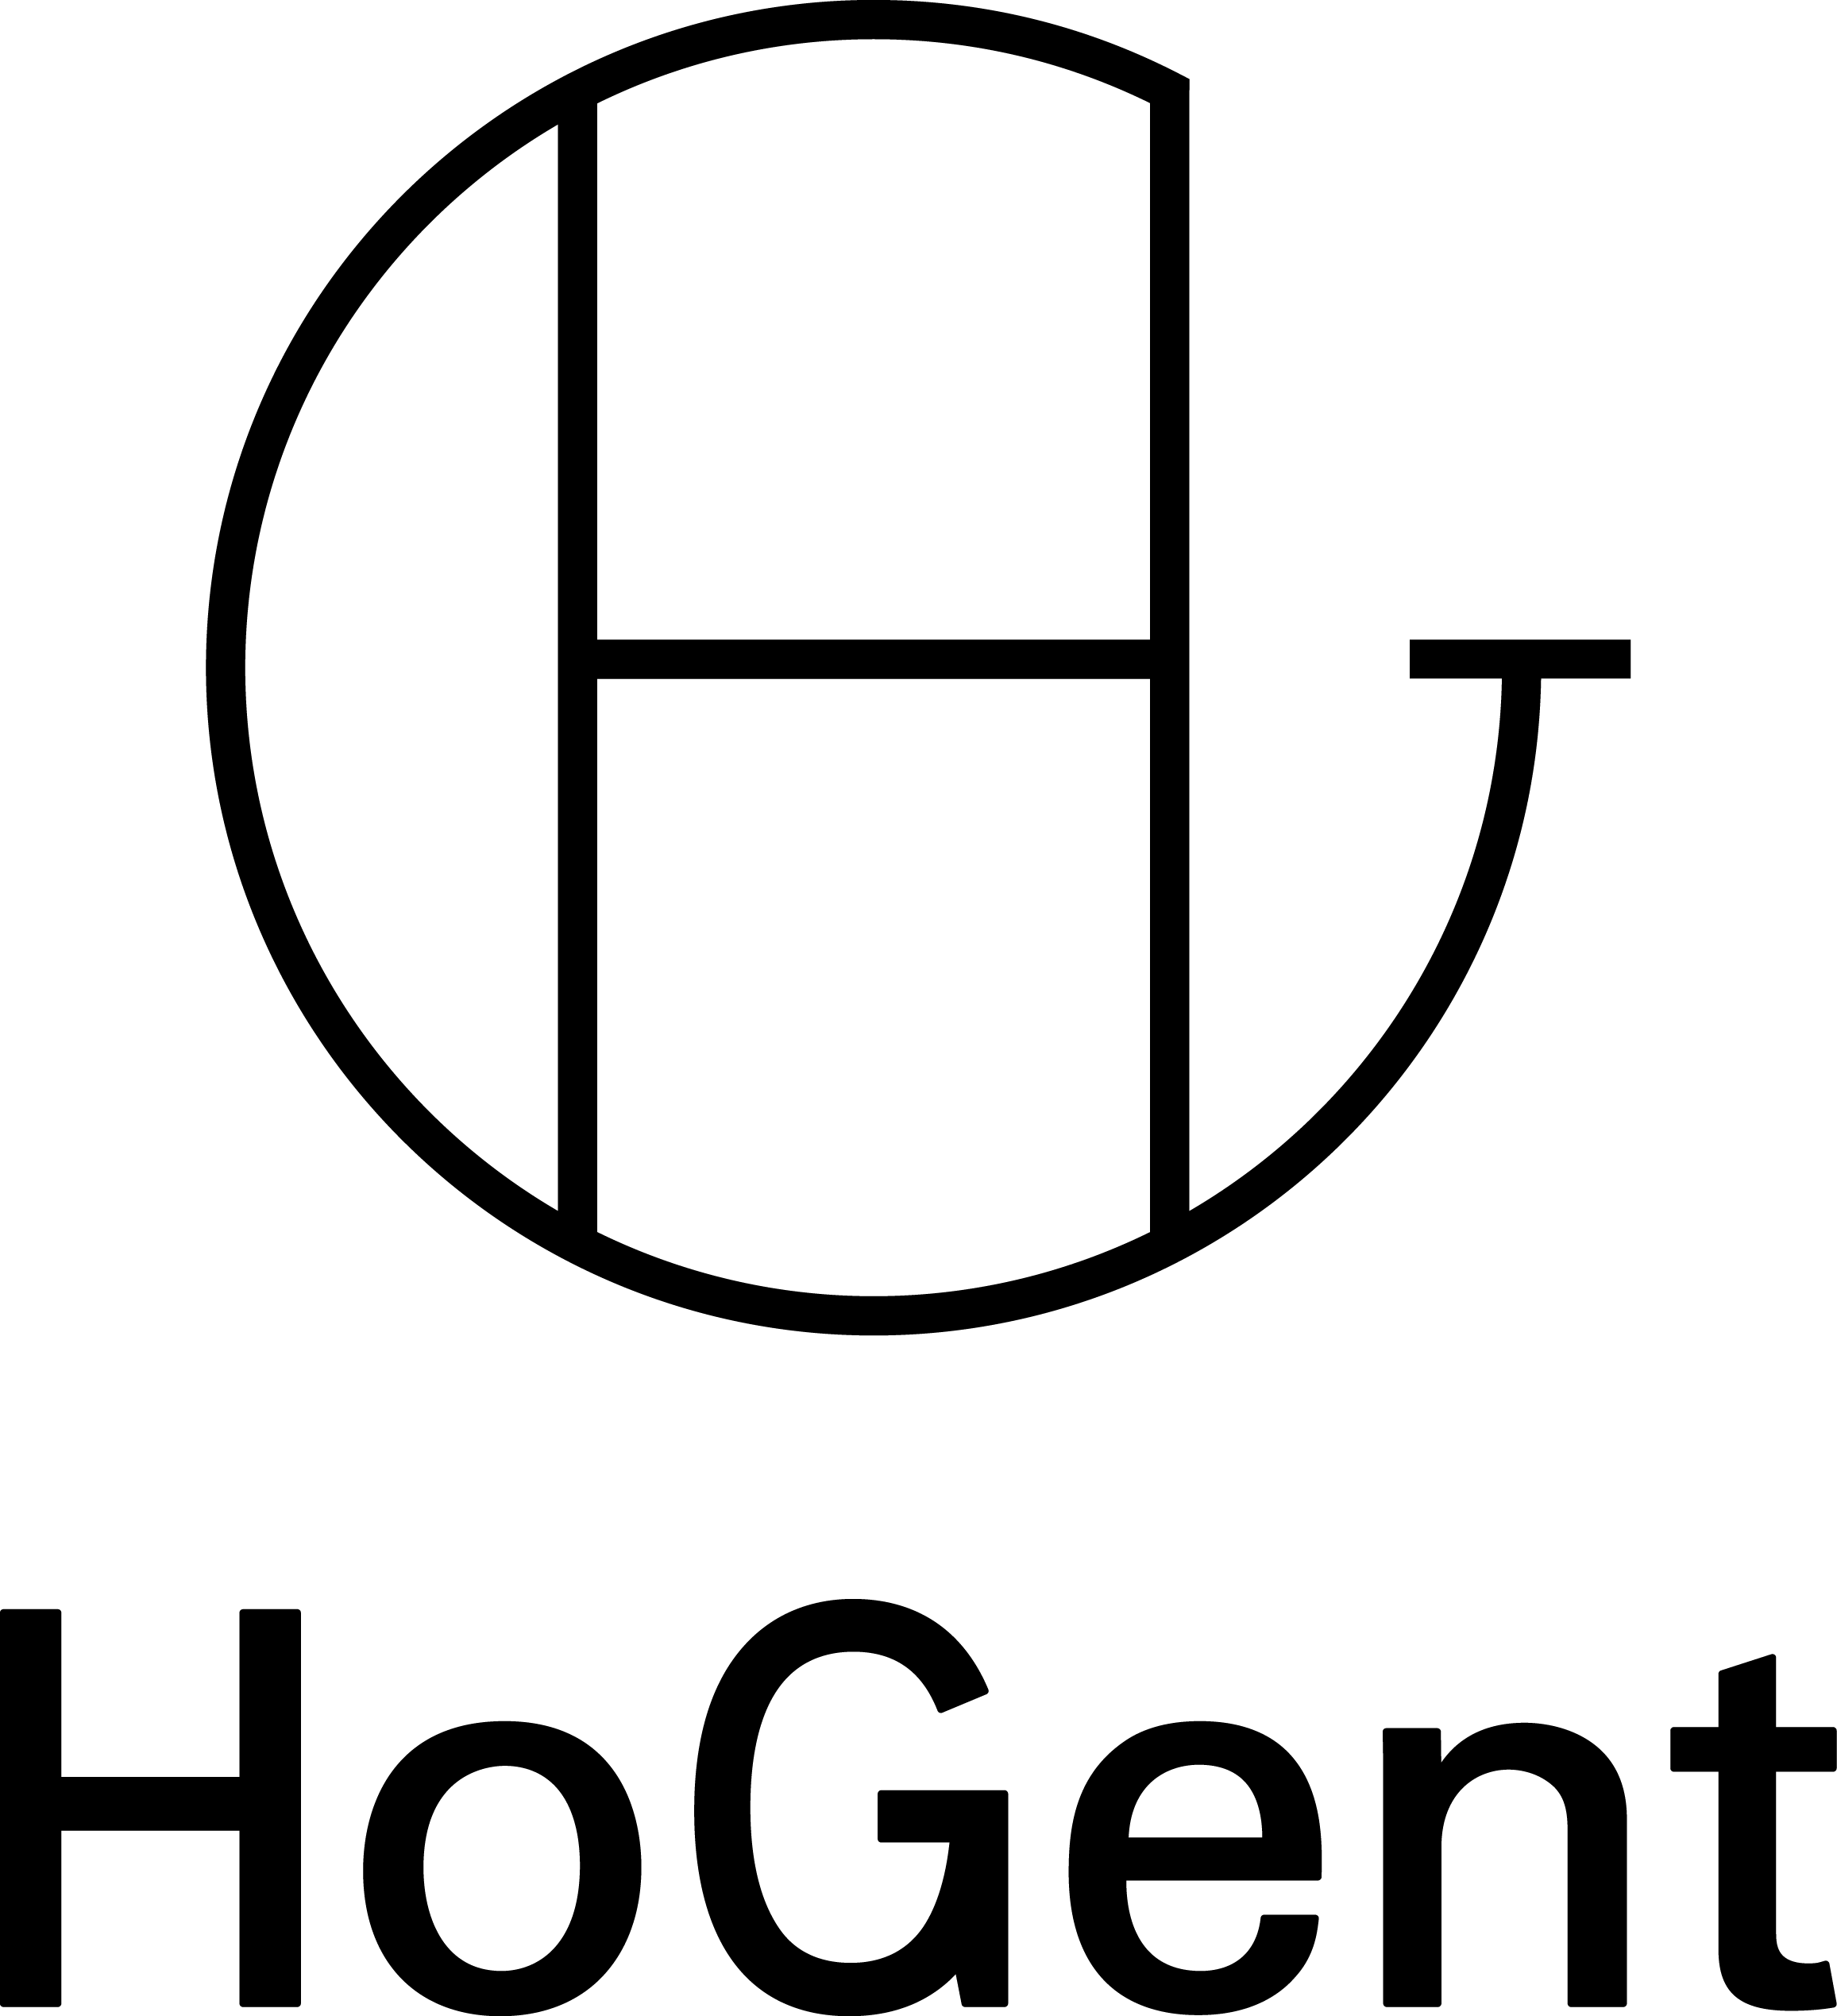
\includegraphics[width=2.5cm]{img/HG-beeldmerk-woordmerk}\\[.5cm]
    Faculteit Bedrijf en Organisatie\\[3cm]
    \titel
    \vfill
    \student\\[3.5cm]
    Scriptie voorgedragen tot het bekomen van de graad van\\professionele bachelor in de toegepaste informatica\\[2cm]
    Promotor:\\
    \promotor\\
    \ifdefempty{\copromotor}{\vspace{2.5cm}}{Co-promotor:\\\copromotor\\[2.5cm]}
    Instelling: \instelling\\[.5cm]
    Academiejaar: \academiejaar\\[.5cm]
    \ifcase \examenperiode \or Eerste \or Tweede \else Derde \fi examenperiode
    \endgroup

  \end{center}
  \restoregeometry
\end{titlepage}
  \emptypage
\begin{titlepage}
  \newgeometry{top=5.35cm,bottom=1.5cm,left=1.5cm,right=1.5cm}
  \begin{center}

    \begingroup
    \rmfamily
    \IfLanguageName{dutch}{Faculteit Bedrijf en Organisatie}{Faculty of Business and Information Management}\\[3cm]
    \titel
    \vfill
    \student\\[3.5cm]
    \IfLanguageName{dutch}{Scriptie voorgedragen tot het bekomen van de graad van\\professionele bachelor in de toegepaste informatica}{Thesis submitted in partial fulfilment of the requirements for the degree of\\professional bachelor of applied computer science}\\[2cm]
    Promotor:\\
    \promotor\\
    \ifdefempty{\copromotor}{\vspace{2.5cm}}{Co-promotor:\\\copromotor\\[2.5cm]}
    \IfLanguageName{dutch}{Instelling}{Institution}: \instelling\\[.5cm]
    \IfLanguageName{dutch}{Academiejaar}{Academic year}: \academiejaar\\[.5cm]
    \IfLanguageName{dutch}{%
    \ifcase \examenperiode \or Eerste \or Tweede \else Derde \fi examenperiode}{%
    \ifcase \examenperiode \or First \or Second \else Third \fi examination period}
    \endgroup

  \end{center}
  \restoregeometry
\end{titlepage}
}

%----------------------------------------------------------------------------------------
%	BIBLIOGRAPHY AND INDEX
%----------------------------------------------------------------------------------------

\usepackage[style=apa,backend=biber]{biblatex}
\usepackage{csquotes}
\DeclareLanguageMapping{dutch}{dutch-apa}
\addbibresource{bachproef-tin.bib} % BibTeX bibliography file
\addbibresource{../voorstel/voorstel.bib}
\defbibheading{bibempty}{}

\usepackage{calc} % For simpler calculation - used for spacing the index letter headings correctly
\usepackage{makeidx} % Required to make an index
\makeindex % Tells LaTeX to create the files required for indexing

%----------------------------------------------------------------------------------------
%	MAIN TABLE OF CONTENTS
%----------------------------------------------------------------------------------------

\usepackage{titletoc} % Required for manipulating the table of contents

\contentsmargin{0cm} % Removes the default margin

% Part text styling
\titlecontents{part}[0cm]
{\addvspace{20pt}\centering\large\bfseries}
{}
{}
{}

% Chapter text styling
\titlecontents{chapter}[1.25cm] % Indentation
{\addvspace{12pt}\large\sffamily\bfseries} % Spacing and font options for chapters
{\color{maincolor!60}\contentslabel[\Large\thecontentslabel]{1.25cm}\color{maincolor}} % Chapter number
{\color{maincolor}}
{\color{maincolor!60}\normalsize\;\titlerule*[.5pc]{.}\;\thecontentspage} % Page number

% Section text styling
\titlecontents{section}[1.25cm] % Indentation
{\addvspace{3pt}\sffamily\bfseries} % Spacing and font options for sections
{\contentslabel[\thecontentslabel]{1.25cm}} % Section number
{}
{\hfill\color{black}\thecontentspage} % Page number
[]

% Subsection text styling
\titlecontents{subsection}[1.25cm] % Indentation
{\addvspace{1pt}\sffamily\small} % Spacing and font options for subsections
{\contentslabel[\thecontentslabel]{1.25cm}} % Subsection number
{}
{\ \titlerule*[.5pc]{.}\;\thecontentspage} % Page number
[]

% List of figures
\titlecontents{figure}[0em]
{\addvspace{-5pt}\sffamily}
{\thecontentslabel\hspace*{1em}}
{}
{\ \titlerule*[.5pc]{.}\;\thecontentspage}
[]

% List of tables
\titlecontents{table}[0em]
{\addvspace{-5pt}\sffamily}
{\thecontentslabel\hspace*{1em}}
{}
{\ \titlerule*[.5pc]{.}\;\thecontentspage}
[]

%----------------------------------------------------------------------------------------
%	MINI TABLE OF CONTENTS IN PART HEADS
%----------------------------------------------------------------------------------------

% Chapter text styling
\titlecontents{lchapter}[0em] % Indenting
{\addvspace{15pt}\large\sffamily\bfseries} % Spacing and font options for chapters
{\color{maincolor}\contentslabel[\Large\thecontentslabel]{1.25cm}\color{maincolor}} % Chapter number
{}
{\color{maincolor}\normalsize\sffamily\bfseries\;\titlerule*[.5pc]{.}\;\thecontentspage} % Page number

% Section text styling
\titlecontents{lsection}[0em] % Indenting
{\sffamily\small} % Spacing and font options for sections
{\contentslabel[\thecontentslabel]{1.25cm}} % Section number
{}
{}

% Subsection text styling
\titlecontents{lsubsection}[.5em] % Indentation
{\normalfont\footnotesize\sffamily} % Font settings
{}
{}
{}

%----------------------------------------------------------------------------------------
%	PAGE HEADERS
%----------------------------------------------------------------------------------------

\usepackage{fancyhdr} % Required for header and footer configuration

\pagestyle{fancy}
\renewcommand{\chaptermark}[1]{\markboth{\sffamily\normalsize\bfseries\chaptername\ \thechapter.\ #1}{}} % Chapter text font settings
\renewcommand{\sectionmark}[1]{\markright{\sffamily\normalsize\thesection\hspace{5pt}#1}{}} % Section text font settings
\fancyhf{} \fancyhead[LE,RO]{\sffamily\normalsize\thepage} % Font setting for the page number in the header
\fancyhead[LO]{\rightmark} % Print the nearest section name on the left side of odd pages
\fancyhead[RE]{\leftmark} % Print the current chapter name on the right side of even pages
\renewcommand{\headrulewidth}{0.5pt} % Width of the rule under the header
\addtolength{\headheight}{2.5pt} % Increase the spacing around the header slightly
\renewcommand{\footrulewidth}{0pt} % Removes the rule in the footer
\fancypagestyle{plain}{\fancyhead{}\renewcommand{\headrulewidth}{0pt}} % Style for when a plain pagestyle is specified

% Removes the header from odd empty pages at the end of chapters
\makeatletter
\renewcommand{\cleardoublepage}{
\clearpage\ifodd\c@page\else
\hbox{}
\vspace*{\fill}
\thispagestyle{empty}
\newpage
\fi}

%----------------------------------------------------------------------------------------
%	THEOREM STYLES
%----------------------------------------------------------------------------------------

\usepackage{amsmath,amsfonts,amssymb,amsthm} % For math equations, theorems, symbols, etc

\newcommand{\intoo}[2]{\mathopen{]}#1\,;#2\mathclose{[}}
\newcommand{\ud}{\mathop{\mathrm{{}d}}\mathopen{}}
\newcommand{\intff}[2]{\mathopen{[}#1\,;#2\mathclose{]}}
\newtheorem{notation}{Notation}[chapter]

% Boxed/framed environments
\newtheoremstyle{maincolornumbox}% % Theorem style name
{0pt}% Space above
{0pt}% Space below
{\normalfont}% % Body font
{}% Indent amount
{\small\bf\sffamily\color{maincolor}}% % Theorem head font
{\;}% Punctuation after theorem head
{0.25em}% Space after theorem head
{\small\sffamily\color{maincolor}\thmname{#1}\nobreakspace\thmnumber{\@ifnotempty{#1}{}\@upn{#2}}% Theorem text (e.g. Theorem 2.1)
\thmnote{\nobreakspace\the\thm@notefont\sffamily\bfseries\color{black}---\nobreakspace#3.}} % Optional theorem note
\renewcommand{\qedsymbol}{$\blacksquare$}% Optional qed square

\newtheoremstyle{blacknumex}% Theorem style name
{5pt}% Space above
{5pt}% Space below
{\normalfont}% Body font
{} % Indent amount
{\small\bf\sffamily}% Theorem head font
{\;}% Punctuation after theorem head
{0.25em}% Space after theorem head
{\small\sffamily{\tiny\ensuremath{\blacksquare}}\nobreakspace\thmname{#1}\nobreakspace\thmnumber{\@ifnotempty{#1}{}\@upn{#2}}% Theorem text (e.g. Theorem 2.1)
\thmnote{\nobreakspace\the\thm@notefont\sffamily\bfseries---\nobreakspace#3.}}% Optional theorem note

\newtheoremstyle{blacknumbox} % Theorem style name
{0pt}% Space above
{0pt}% Space below
{\normalfont}% Body font
{}% Indent amount
{\small\bf\sffamily}% Theorem head font
{\;}% Punctuation after theorem head
{0.25em}% Space after theorem head
{\small\sffamily\thmname{#1}\nobreakspace\thmnumber{\@ifnotempty{#1}{}\@upn{#2}}% Theorem text (e.g. Theorem 2.1)
\thmnote{\nobreakspace\the\thm@notefont\sffamily\bfseries---\nobreakspace#3.}}% Optional theorem note

% Non-boxed/non-framed environments
\newtheoremstyle{maincolornum}% % Theorem style name
{5pt}% Space above
{5pt}% Space below
{\normalfont}% % Body font
{}% Indent amount
{\small\bf\sffamily\color{maincolor}}% % Theorem head font
{\;}% Punctuation after theorem head
{0.25em}% Space after theorem head
{\small\sffamily\color{maincolor}\thmname{#1}\nobreakspace\thmnumber{\@ifnotempty{#1}{}\@upn{#2}}% Theorem text (e.g. Theorem 2.1)
\thmnote{\nobreakspace\the\thm@notefont\sffamily\bfseries\color{black}---\nobreakspace#3.}} % Optional theorem note
\renewcommand{\qedsymbol}{$\blacksquare$}% Optional qed square
\makeatother

% Defines the theorem text style for each type of theorem to one of the three styles above
\newcounter{dummy}
\numberwithin{dummy}{section}
\theoremstyle{maincolornumbox}
\newtheorem{theoremeT}[dummy]{Theorem}
\newtheorem{problem}{Problem}[chapter]
\newtheorem{exerciseT}{Exercise}[chapter]
\theoremstyle{blacknumex}
\newtheorem{exampleT}{Example}[chapter]
\theoremstyle{blacknumbox}
\newtheorem{vocabulary}{Vocabulary}[chapter]
\newtheorem{definitionT}{Definition}[section]
\newtheorem{corollaryT}[dummy]{Corollary}
\theoremstyle{maincolornum}
\newtheorem{proposition}[dummy]{Proposition}

%----------------------------------------------------------------------------------------
%	DEFINITION OF COLORED BOXES
%----------------------------------------------------------------------------------------

\RequirePackage[framemethod=default]{mdframed} % Required for creating the theorem, definition, exercise and corollary boxes

% Theorem box
\newmdenv[skipabove=7pt,
skipbelow=7pt,
backgroundcolor=black!5,
linecolor=maincolor,
innerleftmargin=5pt,
innerrightmargin=5pt,
innertopmargin=5pt,
leftmargin=0cm,
rightmargin=0cm,
innerbottommargin=5pt]{tBox}

% Exercise box
\newmdenv[skipabove=7pt,
skipbelow=7pt,
rightline=false,
leftline=true,
topline=false,
bottomline=false,
backgroundcolor=maincolor!10,
linecolor=maincolor,
innerleftmargin=5pt,
innerrightmargin=5pt,
innertopmargin=5pt,
innerbottommargin=5pt,
leftmargin=0cm,
rightmargin=0cm,
linewidth=4pt]{eBox}

% Definition box
\newmdenv[skipabove=7pt,
skipbelow=7pt,
rightline=false,
leftline=true,
topline=false,
bottomline=false,
linecolor=maincolor,
innerleftmargin=5pt,
innerrightmargin=5pt,
innertopmargin=0pt,
leftmargin=0cm,
rightmargin=0cm,
linewidth=4pt,
innerbottommargin=0pt]{dBox}

% Corollary box
\newmdenv[skipabove=7pt,
skipbelow=7pt,
rightline=false,
leftline=true,
topline=false,
bottomline=false,
linecolor=gray,
backgroundcolor=black!5,
innerleftmargin=5pt,
innerrightmargin=5pt,
innertopmargin=5pt,
leftmargin=0cm,
rightmargin=0cm,
linewidth=4pt,
innerbottommargin=5pt]{cBox}

% Creates an environment for each type of theorem and assigns it a theorem text style from the "Theorem Styles" section above and a colored box from above
\newenvironment{theorem}{\begin{tBox}\begin{theoremeT}}{\end{theoremeT}\end{tBox}}
\newenvironment{exercise}{\begin{eBox}\begin{exerciseT}}{\hfill{\color{maincolor}\tiny\ensuremath{\blacksquare}}\end{exerciseT}\end{eBox}}
\newenvironment{definition}{\begin{dBox}\begin{definitionT}}{\end{definitionT}\end{dBox}}
\newenvironment{example}{\begin{exampleT}}{\hfill{\tiny\ensuremath{\blacksquare}}\end{exampleT}}
\newenvironment{corollary}{\begin{cBox}\begin{corollaryT}}{\end{corollaryT}\end{cBox}}

%----------------------------------------------------------------------------------------
%	REMARK ENVIRONMENT
%----------------------------------------------------------------------------------------

\newenvironment{remark}{\par\vspace{10pt}\small % Vertical white space above the remark and smaller font size
\begin{list}{}{
\leftmargin=35pt % Indentation on the left
\rightmargin=25pt}\item\ignorespaces % Indentation on the right
\makebox[-2.5pt]{\begin{tikzpicture}[overlay]
\node[draw=maincolor!60,line width=1pt,circle,fill=maincolor!25,font=\sffamily\bfseries,inner sep=2pt,outer sep=0pt] at (-15pt,0pt){\textcolor{maincolor}{R}};\end{tikzpicture}} % Orange R in a circle
\advance\baselineskip -1pt}{\end{list}\vskip5pt} % Tighter line spacing and white space after remark

%----------------------------------------------------------------------------------------
%	SECTION NUMBERING IN THE MARGIN
%----------------------------------------------------------------------------------------

\makeatletter
\renewcommand{\@seccntformat}[1]{\llap{\textcolor{maincolor}{\csname the#1\endcsname}\hspace{1em}}}
\renewcommand{\section}{\@startsection{section}{1}{\z@}
{-4ex \@plus -1ex \@minus -.4ex}
{1ex \@plus.2ex }
{\normalfont\large\sffamily\bfseries}}
\renewcommand{\subsection}{\@startsection {subsection}{2}{\z@}
{-3ex \@plus -0.1ex \@minus -.4ex}
{0.5ex \@plus.2ex }
{\normalfont\sffamily\bfseries}}
\renewcommand{\subsubsection}{\@startsection {subsubsection}{3}{\z@}
{-2ex \@plus -0.1ex \@minus -.2ex}
{.2ex \@plus.2ex }
{\normalfont\small\sffamily\bfseries}}
\renewcommand\paragraph{\@startsection{paragraph}{4}{\z@}
{-2ex \@plus-.2ex \@minus .2ex}
{.1ex}
{\normalfont\small\sffamily\bfseries}}

%----------------------------------------------------------------------------------------
%	PART HEADINGS
%----------------------------------------------------------------------------------------

% numbered part in the table of contents
\newcommand{\@mypartnumtocformat}[2]{%
\setlength\fboxsep{0pt}%
\noindent\colorbox{maincolor!20}{\strut\parbox[c][.7cm]{\ecart}{\color{maincolor!70}\Large\sffamily\bfseries\centering#1}}\hskip\esp\colorbox{maincolor!40}{\strut\parbox[c][.7cm]{\linewidth-\ecart-\esp}{\Large\sffamily\centering#2}}}%
%%%%%%%%%%%%%%%%%%%%%%%%%%%%%%%%%%
% unnumbered part in the table of contents
\newcommand{\@myparttocformat}[1]{%
\setlength\fboxsep{0pt}%
\noindent\colorbox{maincolor!40}{\strut\parbox[c][.7cm]{\linewidth}{\Large\sffamily\centering#1}}}%
%%%%%%%%%%%%%%%%%%%%%%%%%%%%%%%%%%
\newlength\esp
\setlength\esp{4pt}
\newlength\ecart
\setlength\ecart{1.2cm-\esp}
\newcommand{\thepartimage}{}%
\newcommand{\partimage}[1]{\renewcommand{\thepartimage}{#1}}%
\def\@part[#1]#2{%
\ifnum \c@secnumdepth >-2\relax%
\refstepcounter{part}%
\addcontentsline{toc}{part}{\texorpdfstring{\protect\@mypartnumtocformat{\thepart}{#1}}{\partname~\thepart\ ---\ #1}}
\else%
\addcontentsline{toc}{part}{\texorpdfstring{\protect\@myparttocformat{#1}}{#1}}%
\fi%
\startcontents%
\markboth{}{}%
{\thispagestyle{empty}%
\begin{tikzpicture}[remember picture,overlay]%
\node at (current page.north west){\begin{tikzpicture}[remember picture,overlay]%
\fill[maincolor!20](0cm,0cm) rectangle (\paperwidth,-\paperheight);
\node[anchor=north] at (4cm,-3.25cm){\color{maincolor!40}\fontsize{220}{100}\sffamily\bfseries\@Roman\c@part};
\node[anchor=south east] at (\paperwidth-1cm,-\paperheight+1cm){\parbox[t][][t]{8.5cm}{
\printcontents{l}{0}{\setcounter{tocdepth}{1}}%
}};
\node[anchor=north east] at (\paperwidth-1.5cm,-3.25cm){\parbox[t][][t]{15cm}{\strut\raggedleft\color{white}\fontsize{30}{30}\sffamily\bfseries#2}};
\end{tikzpicture}};
\end{tikzpicture}}%
\@endpart}
\def\@spart#1{%
\startcontents%
\phantomsection
{\thispagestyle{empty}%
\begin{tikzpicture}[remember picture,overlay]%
\node at (current page.north west){\begin{tikzpicture}[remember picture,overlay]%
\fill[maincolor!20](0cm,0cm) rectangle (\paperwidth,-\paperheight);
\node[anchor=north east] at (\paperwidth-1.5cm,-3.25cm){\parbox[t][][t]{15cm}{\strut\raggedleft\color{white}\fontsize{30}{30}\sffamily\bfseries#1}};
\end{tikzpicture}};
\end{tikzpicture}}
\addcontentsline{toc}{part}{\texorpdfstring{%
\setlength\fboxsep{0pt}%
\noindent\protect\colorbox{maincolor!40}{\strut\protect\parbox[c][.7cm]{\linewidth}{\Large\sffamily\protect\centering #1\quad\mbox{}}}}{#1}}%
\@endpart}
\def\@endpart{\vfil\newpage
\if@twoside
\if@openright
\null
\thispagestyle{empty}%
\newpage
\fi
\fi
\if@tempswa
\twocolumn
\fi}

%----------------------------------------------------------------------------------------
%	CHAPTER HEADINGS
%----------------------------------------------------------------------------------------

% A switch to conditionally include a picture, implemented by  Christian Hupfer
\newif\ifusechapterimage
\usechapterimagetrue
\newcommand{\thechapterimage}{}%
\newcommand{\chapterimage}[1]{\ifusechapterimage\renewcommand{\thechapterimage}{#1}\fi}%
\def\@makechapterhead#1{%
{\parindent \z@ \raggedright \normalfont
\ifnum \c@secnumdepth >\m@ne
\if@mainmatter
\begin{tikzpicture}[remember picture,overlay]
\node at (current page.north west)
{\begin{tikzpicture}[remember picture,overlay]
\node[anchor=north west,inner sep=0pt] at (0,0) {\ifusechapterimage\includegraphics[width=\paperwidth]{\thechapterimage}\fi};
\draw[anchor=west] (\Gm@lmargin,-9cm) node [line width=2pt,rounded corners=15pt,draw=maincolor,fill=white,fill opacity=0.5,inner sep=15pt]{\strut\makebox[22cm]{}};
\draw[anchor=west] (\Gm@lmargin+.3cm,-9cm) node {\huge\sffamily\bfseries\color{black}\thechapter. #1\strut};
\end{tikzpicture}};
\end{tikzpicture}
\else
\begin{tikzpicture}[remember picture,overlay]
\node at (current page.north west)
{\begin{tikzpicture}[remember picture,overlay]
\node[anchor=north west,inner sep=0pt] at (0,0) {\ifusechapterimage\includegraphics[width=\paperwidth]{\thechapterimage}\fi};
\draw[anchor=west] (\Gm@lmargin,-9cm) node [line width=2pt,rounded corners=15pt,draw=maincolor,fill=white,fill opacity=0.5,inner sep=15pt]{\strut\makebox[22cm]{}};
\draw[anchor=west] (\Gm@lmargin+.3cm,-9cm) node {\huge\sffamily\bfseries\color{black}#1\strut};
\end{tikzpicture}};
\end{tikzpicture}
\fi\fi\par\vspace*{270\p@}}}

%-------------------------------------------

\def\@makeschapterhead#1{%
\begin{tikzpicture}[remember picture,overlay]
\node at (current page.north west)
{\begin{tikzpicture}[remember picture,overlay]
\node[anchor=north west,inner sep=0pt] at (0,0) {\ifusechapterimage\includegraphics[width=\paperwidth]{\thechapterimage}\fi};
\draw[anchor=west] (\Gm@lmargin,-9cm) node [line width=2pt,rounded corners=15pt,draw=maincolor,fill=white,fill opacity=0.5,inner sep=15pt]{\strut\makebox[22cm]{}};
\draw[anchor=west] (\Gm@lmargin+.3cm,-9cm) node {\huge\sffamily\bfseries\color{black}#1\strut};
\end{tikzpicture}};
\end{tikzpicture}
\par\vspace*{270\p@}}
\makeatother

%----------------------------------------------------------------------------------------
%	HYPERLINKS IN THE DOCUMENTS
%----------------------------------------------------------------------------------------

\usepackage{hyperref}
\hypersetup{hidelinks,backref=true,pagebackref=true,hyperindex=true,colorlinks=false,breaklinks=true,urlcolor= maincolor,bookmarks=true,bookmarksopen=false,pdftitle={Title},pdfauthor={Author}}
\usepackage{bookmark}
\bookmarksetup{
open,
numbered,
addtohook={%
\ifnum\bookmarkget{level}=0 % chapter
\bookmarksetup{bold}%
\fi
\ifnum\bookmarkget{level}=-1 % part
\bookmarksetup{color=maincolor,bold}%
\fi
}
}

%----------------------------------------------------------------------------------------
%	Java source code
%----------------------------------------------------------------------------------------

% Commando voor invoegen Java-broncodebestanden (dank aan Niels Corneille)
% Gebruik:
%   \codefragment{source/MijnKlasse.java}{Uitleg bij de code}
%
% Je kan dit aanpassen aan de taal die je zelf het meeste gebruikt in je
% bachelorproef.
\newcommand{\codefragment}[2]{ \lstset{%
  language=java,
  breaklines=true,
  float=th,
  caption={#2},
  basicstyle=\scriptsize,
  frame=single,
  extendedchars=\true
}
\lstinputlisting{#1}}

% Leeg blad
\newcommand{\emptypage}{%
\newpage
\thispagestyle{empty}
\mbox{}
\newpage
}


%%---------- Documenteigenschappen --------------------------------------------
%% TODO: Vul dit aan met je eigen info:

% Je eigen naam
\newcommand{\student}{Coppens Robin}

% De naam van je promotor (lector van de opleiding)
\newcommand{\promotor}{Smits Lieven }

% De naam van je co-promotor. Als je promotor ook je opdrachtgever is en je
% dus ook inhoudelijk begeleidt (en enkel dan!), mag je dit leeg laten.
\newcommand{\copromotor}{Smiedts Diaz}

% Indien je bachelorproef in opdracht van/in samenwerking met een bedrijf of
% externe organisatie geschreven is, geef je hier de naam. Zoniet laat je dit
% zoals het is.
\newcommand{\instelling}{Into Data}

% De titel van het rapport/bachelorproef
\newcommand{\titel}{Hoe kan machine learning klantenbinding of churn prevention faciliteren?}

% Datum van indienen (gebruik telkens de deadline, ook al geef je eerder af)
\newcommand{\datum}{27 mei 2016}

% Academiejaar
\newcommand{\academiejaar}{2017-2018}

% Examenperiode
%  - 1e semester = 1e examenperiode => 1
%  - 2e semester = 2e examenperiode => 2
%  - tweede zit  = 3e examenperiode => 3
\newcommand{\examenperiode}{1}

%%=============================================================================
%% Inhoud document
%%=============================================================================

\begin{document}

%---------- Taalselectie ------------------------------------------------------
% Als je je bachelorproef in het Engels schrijft, haal dan onderstaande regel
% uit commentaar. Let op: de tekst op de voorkaft blijft in het Nederlands, en
% dat is ook de bedoeling!

%\selectlanguage{english}

%---------- Titelblad ---------------------------------------------------------
\inserttitlepage

%---------- Samenvatting, voorwoord -------------------------------------------
\usechapterimagefalse
%%=============================================================================
%% Voorwoord
%%=============================================================================

\chapter*{Woord vooraf}
\label{ch:voorwoord}

%% TODO:
In het laatste jaar toegepaste informatica aan de Hogeschool Gent wordt er verwacht dat elke student een Bachelorproef schrijft over een onderwerp dat relevant is voor de opleiding. 
Het idee was om een onderzoek te doen op welke manier en met welke data we via Machine Learning geautomatiseerd kunnen afleiden wie op een bepaald moment een firma wil verlaten of een bepaalde service zal opzeggen. Hierbij hebben we volgende onderzoeksvragen. Welke tools/ oplossingen met Machine Learning zijn er nu op de markt die klantbinding/churn prevention faciliteren. Welke tools kan men zelf gebruiken om zelf een oplossing te bouwen.
Het idee van het gekozen onderwerp komt van meneer Diaz Smiedts, werkende bij IntoData. Hem wil ik bedanken om de verantwoordelijkheid van co-promotor op zich te nemen en om mij een onderwerp voor te stellen als Bachelorproef. Een goed Bachelorproef is niet makkelijk te vinden.
Meneer Lievens Smits wil ik ook bedanken voor begeleiding gedurende deze periode als promotor van deze Bachelorproef. 



%%=============================================================================
%% Samenvatting
%%=============================================================================

% TODO: De "abstract" of samenvatting is een kernachtige (~ 1 blz. voor een
% thesis) synthese van het document.
%
% Deze aspecten moeten zeker aan bod komen:
% - Context: waarom is dit werk belangrijk?
% - Nood: waarom moest dit onderzocht worden?
% - Taak: wat heb je precies gedaan?
% - Object: wat staat in dit document geschreven?
% - Resultaat: wat was het resultaat?
% - Conclusie: wat is/zijn de belangrijkste conclusie(s)?
% - Perspectief: blijven er nog vragen open die in de toekomst nog kunnen
%    onderzocht worden? Wat is een mogelijk vervolg voor jouw onderzoek?
%
% LET OP! Een samenvatting is GEEN voorwoord!

%%---------- Nederlandse samenvatting -----------------------------------------
%
% TODO: Als je je bachelorproef in het Engels schrijft, moet je eerst een
% Nederlandse samenvatting invoegen. Haal daarvoor onderstaande code uit
% commentaar.
% Wie zijn bachelorproef in het Nederlands schrijft, kan dit negeren, de inhoud
% wordt niet in het document ingevoegd.

\IfLanguageName{english}{%
\selectlanguage{dutch}
\chapter*{Samenvatting}
Elk bedrijf doet veel moeite om klanten te werven, maar verliest de groep uit het oog die reeds klant is, Nochtans is customer-binding, customer retention en churn prevention even belangrijk. Maar ook dit vergt heel wat tijd en energie en wordt dikwijls pas in een laatste fase bekeken in het klanten proces. Machine Learning kan deze taak eventueel geautomatiseerd uitvoeren. Hierbij doet men dus een onderzoek op welke manier en met welke data we via Machine Learning geautomatiseerd kunnen afleiden wie op een bepaalde moment een firma zal verlaten of bepaalde service zal opzeggen.

In deze Bachelorproef heeft men op basis van sites en algemeen verkregen documentatie bekeken wat de mogelijkheden zijn om dit onderzoek te volbrengen
Hierbij is men onder andere tot de conclusie gekomen dat klanten meer op emotioneel niveau kijken of ze bij een bepaalde firma blijven. Maar dit is niet van toepassing voor een aankoop op een site. Dus heeft men zich dan gebaseerd op het rationeel niveau. 
Na de literatuurstudie begon men de onderzoeksvragen elk apart te beantwoorden.
Men heeft gezien dat er nog andere technologieën zijn die Machine Learning gebruiken voor churn prevention. Namelijk: Dataiku, Databricks en de IBM Watson Analytics. Men heeft de verschillende soorten tools onderzocht en bekeken welke tools men het beste zou gebruiken voor zelf een Machine learning model te maken. De conclusie was dat we een library, API, local tool gaan gebruiken. Hieronder hebben we 2 tools gevonden op het internet :DeepLearningforj en TenserFlow. Vervolgens hebben we gekozen voor TenserFlow. Vanwege xyz. Men heeft onderzocht wat voor dataset men nodig had om het model op te trainen. Gelukkig was er een model dat men kon vinden en konden gebruiken. De Telco-Customer-Churn dataset. 

\selectlanguage{english}
}{}

%%---------- Samenvatting -----------------------------------------------------
% De samenvatting in de hoofdtaal van het document

\chapter*{\IfLanguageName{dutch}{Samenvatting}{Abstract}}

\lipsum[1-4]


%---------- Inhoudstafel ------------------------------------------------------
\pagestyle{empty} % No headers
\tableofcontents % Print the table of contents itself
\cleardoublepage % Forces the first chapter to start on an odd page so it's on the right
\pagestyle{fancy} % Print headers again

%---------- Lijst figuren, afkortingen, ... -----------------------------------

% Indien gewenst kan je hier een lijst van figuren/tabellen opgeven. Geef in
% dat geval je figuren/tabellen altijd een korte beschrijving:
%
%  \caption[korte beschrijving]{uitgebreide beschrijving}

\listoffigures
\listoftables

% Als je een lijst van afkortingen of termen wil toevoegen, dan hoort die
% hier thuis. Gebruik bijvoorbeeld de ``glossaries'' package.
% https://www.sharelatex.com/learn/Glossaries

%%---------- Kern -------------------------------------------------------------

%%=============================================================================
%% Inleiding
%%=============================================================================

\chapter{Inleiding}
\label{ch:inleiding}



\section{Probleemstelling}
\label{sec:probleemstelling en context}
Elk bedrijf doet veel moeite om klanten te werven, maar verliest de groep uit het oog die reeds klant is, Nochtans is customer-binding, customer retention en churn prevention even belangrijk. Maar ook dit vergt heel wat tijd en energie en wordt dikwijls pas in een laatste fase bekeken in het klanten proces. Machine Learning kan deze taak eventueel geautomatiseerd uitvoeren. Hierbij doet men dus een onderzoek op welke manier en met welke data we via Machine Learning geautomatiseerd kunnen aflijden wie op een bepaald moment een firma zal verlaten of bepaalde service zal opzeggen.

\section{Onderzoeksvraag}
\label{sec:Doelstelling en onderzoeksvragen}

Eerst en vooral gaan we informatie opzoeken over belangrijke termen in deze bachelorproef zoals Churn, Churn prevention, Klantenbinding, Machine Learning, Models, Deep Learning, Datasets. Aan de hand van deze informatie kan men dan kijken hoe men Machine Learning kan gebruiken voor churn of klantenbinding. Om uiteindelijk resultaat te krijgen zullen er eerst en vooral een aantal onderzoeksvragen opgelost worden:


\begin{description}
	\item [Zijn er andere technologieën die Machine Learning reeds toepassen voor churn of klantenbinding?] In deze fase gaan we op zoek gaan naar technologieën die reeds gebruik maken van Machine Learning voor churn of klantenbinding. 
	\item [Welke frameworks, visuele tools en scripting tools heb ik nodig om zelf zo een oplossing te bouwen?] In deze fase gaat men eerst kijken welke soort tools er te vinden zijn, en hoe we deze kunnen onderscheiden. Vervolgens gaat men bekijken welke soort tools het beste van toepassing zouden zijn voor ons onderzoek. Om hierna dan te zoeken naar tools die onder de gekozen soort vallen. En vervolgens een paar van deze te gaan vergelijken .
	\item [Welke data set gaan we gebruiken en hoe verkrijg ik deze data ?] Hier is het de bedoeling dat we eerst weten welke parameters belangrijk zijn voor het voorspellen van een churn, om vervolgens dan een data set zelf te maken of een data set op te zoeken op het web die parameters bevat die het meest aanleunen aan onze gekozen parameters.
	\item [Welk Model dien ik hiervoor op te zetten]Hiervoor gaan we kijken naar de algoritmes die in aanmerking komen voor het model. Vervolgens besluiten welk algoritme we gaan gebruiken.
	\item [Kies ik beter een scripting tool zoals python?]Men gaat onderzoeken waarom in het geval van een model maken, scripting tools beter zijn.
\end{description}


\chapter{Literatuur studie}
\label{ch:Literatuur studie}

% Tip: Begin elk hoofdstuk met een paragraaf inleiding die beschrijft hoe
% dit hoofdstuk past binnen het geheel van de bachelorproef. Geef in het
% bijzonder aan wat de link is met het vorige en volgende hoofdstuk.

% Pas na deze inleidende paragraaf komt de eerste sectiehoofding.

\section{Waarom Machine Learning}
\label{sec:Waarom Machine Learning?}

Machine Learning heeft al meerdere keren zijn kracht en nut laten zien. Zoals in 2015 heeft Google een A.I. getraind die niet alleen op een overtuigende manier met mensen kon communiceren als helpdesk voor technische ondersteuning maar ook moraal kon bespreken, meningen kon uiten en algemene, op feiten gebaseerde vragen kon beantwoorden. Zoals u kan zien op de afbeelding hieronder.

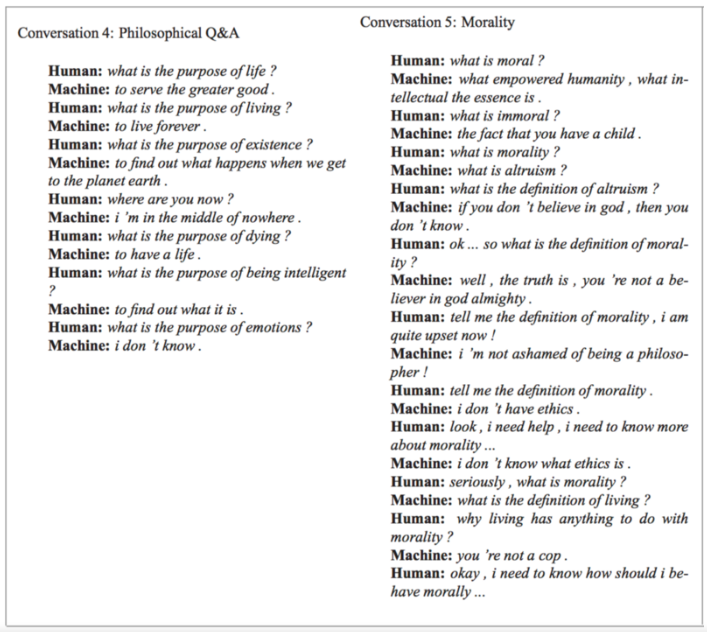
\includegraphics[scale=0.7]{img/MLC}

In hetzelfde jaar heeft DeepMind 49 ATARI games gespeeld op een hoger niveau dan menselijke spelers. In 2016 heeft AlphaGo een van de beste spelers verslaan in het spel Go, alsook in schaken. Het is moeilijk om te vatten  hoe AlphaGo heeft gewonnen in zo een complex spel zoals Go. Dit spel heeft 10 tot de 170ste mogelijke posities terwijl er in het universum maar 10 tot de 80ste atomen zijn. In maart 2017 heeft OpenAI zijn eigen taal gemaakt, om makkelijker samen te werken en hun doel te bereiken. Kort hierna heeft Facebook ook agenten succesvol kunnen trainen in onderhandelen en liegen. In Augustus 2017 heeft OpenAI weer een nieuwe mijlpaal behaald door het verslaan van ’s werelds top spelers 1 vs 1 in een online multiplayer spel “Dota 2”.

Vandaag de dag wordt A.I. gebruikt om evidence-based behandelingsplannen voor kankerpatiënten te ontwerpen, onmiddellijk resultaten van medische tests te analyseren om vervolgens onmiddellijk naar de juiste specialist door te sturen en wetenschappelijk onderzoek uit te voeren voor het ontdekken van geneesmiddelen. In het dagelijkse leven gebeurt het vaker dat machines taken overnemen van mensen. Dus in deze bachelorproef veronderstelt men dat dit ook zo zal zijn bij Machine Learning. 

\section{Klantenbinding}
\label{sec:Klantenbinding}
De eerste vraag die je je moet stellen is, wat is klantenbinding? Dit zijn maatregelen die een bedrijf neemt die ervoor zorgen dat een klant producten blijft kopen van zijn bedrijf. Het bedrijf speelt in op de behoeften van de klant om zo dus een voorkeurspositie te krijgen. De klantenrelatie wordt versterkt en er is een kleinere kans dat de klant gaat overstappen naar de concurrent. “De Klant wordt als het ware een ambassadeur van het bedrijf”

Business-to-Business of B2B marketing concentreert zich op de mate van aanbeveling en niet op het product. Om een voorkeurspositie in het hoofd van de klant te realiseren, kunnen bedrijven de klantenbinding op drie niveaus beïnvloeden.

\begin{description}
	\item [Rationeel niveau]Bij deze vorm van binding gaat het om het creëren van een financieel voordeel. Het verlenen van bijvoorbeeld additionele diensten en beloningen vergroot de kans op positieve respons.
	\item [Sociaal/emotioneel niveau]Sociale binding is een vorm van emotionele binding waar de focus wordt gelegd op de manier van communiceren. Hierbij ligt de focus op het creëren van intensievere contactmomenten. Intensief contact met de klant beïnvloedt de beleving rondom het merk positief en vergroot daardoor de kans op een sterk imago.
	\item [Structureel niveau] Bij structurele binding gaat het om de extra mogelijkheden die het bedrijf biedt bij het leveren van producten en of diensten. Het leveren van bijvoorbeeld maatwerk of unieke producten zorgt ervoor dat de klant een voordeel ziet. Hierbij ligt de nadruk op het inspelen op de wensen en behoeften van de klant.
\end{description}

Mogelijke toepassing op elk van deze niveaus

\begin{description}
	\item [Rationeel niveau] Op rationeel niveau kan er gebruik gemaakt worden van een programma dat telkens een product opzoekt bij de concurrent en dit product dan bij hun bedrijf goedkoper zou maken. Maar dit idee is ook perfect mogelijk te maken zonder het gebruik van Machine Learning. Wat wel nog zou gaan is om aan de hand van klantenvoordelen dat een bedrijf geeft en de response van de klant hierop een model trainen. Zodanig dat er een ideale methodiek is voor klanten.
	\item [Sociaal/emotioneel niveau]Dit niveau is nog te moeilijk om te bereiken met Machine Learning. We kunnen hier misschien wel al een toepassing doen van chatbots en dergelijke. Maar dan raken we niet echt het emotionele aspect van de klant. Of in ieder geval, is dit moeilijker te bespelen. Hiervoor is volgens mij wel nood aan het menselijke contact 
	\item [Structureel niveau] Een mogelijkheid kan zijn dat een dienst-leverancier jou de mogelijkheid biedt om via hen eenvoudig een andere dienst bij te nemen, bv Engie Electrabel(en andere sector genoten) die ook onderhoud aanbieden van CV ketels etc. Geen core business voor hen , maar een structurele meerwaarde om bij de leverancier te blijven omdat die een ander “probleem” uit handen neemt van de klant.
\end{description}

30\% van de klanten wordt overtuigd op rationeel niveau en 70\% van klanten op emotioneel niveau deze cijfers komen van een onderzoek van de Harvard Business Review (HBR bron). Dit is volgens mij correct voor winkels in een winkelstraat of stad. Maar pakweg online schoenen kopen bij Zalando of torfs ga je minder snel beslissen vanuit emotioneel standpunt. Vervolgens zal men zich voor deze Bachelorproef richting op het rationele aspect. 

Wanneer is een klant tevreden? Het gaat hem meer om de klanten die loyaal zijn. Tevreden klanten kunnen nog te rap naar de concurrentie overstappen. Terwijl zeer tevreden klanten onder de naam loyale klanten vallen.

\section{Churn}
\label{sec:Churn}
Wat is churn ? Het is eigenlijk vrij eenvoudig. Churn is wanneer er klanten vertrekken. Dit is iets waar elk bedrijf aan moet werken. Want zonder klanten heb je geen omzet. Ook al krijg je snel genoeg nieuwe klanten. Er moet worden gewerkt aan klanten behouden. Bedrijven kunnen hiervoor gebruik maken van predictive models dat dit gaan voorspellen en uiteindelijk kan het bedrijf hierop dan actie ondernemen.

\textbf{Subscription churn en non-subscription churn}
Er zijn 2 basis types van churn; subscription churn en non subscription churn

We spreken van \textbf{subscription churn} als het bedrijf gebruik maakt van een abonnement voor een bepaalde periode (maandelijks, wekelijks of zelfs dagelijks) en de klanten kiezen ervoor om niet meer terug te komen. Nadat het contract is stopgezet. Is het makkelijk om churn te definiëren , voorspellen. Omdat er een duidelijke beeld is dat men kan maken


\includegraphics[scale=0.7]{img/subscription-churn}

\textbf{Non subscription churn} kan gebeuren wanneer de klant verkiest om op het even welk moment zijn relatie met het bedrijf stop te zetten. Klanten kunnen gelijdelijk aan minder vaak kopen bij het bedrijf. Of ze kunnen plots nooit meer een product/dienst kopen bij het bedrijf.

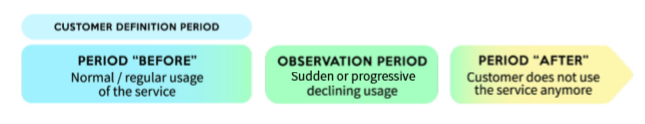
\includegraphics[scale=0.8]{img/non-subscription-churn}

\section{Churn prevention}
\label{sec:Churn prevention}
Nog een belangrijke term in deze Bachelorproef is Churn prevention. Dit is dus eigenlijk het voorkomen dat de klant overstapt naar een concurrent. Customer churn is het getal berekent door het aantal personen die het bedrijf verlaten binnen een gegeven tijds periode. Churn rate is dan eigenlijk een indicator hoe een gegeven bedrijf het doet in zake van het behouden van zijn klanten(SO bron)

Er zijn een aantal manieren om Customer Churn te verminderen. Hiervan noemt men enkel degene op die van toepassing kunnen zijn met machine learning.(SO bron)

\begin{description}
	\item Analyseren \newline
	Het eerste is misschien overbodig om te vermelden maar dit moet zeker gebeuren volgens (SO BRON) Het is belangrijk om te weten waarom een klant het bedrijf verlaat. Dit doet men door bijvoorbeeld te praten met de klant. Hierdoor laat je direct zien dat je het belangrijk vindt om te weten waarom de klant is overgestapt naar de concurrentie. En doe dit zeker niet met surveys. Dit voelt onmenselijk aan en uit nature vermijden we die zaken. Dus echt converseren met mensen zal moeilijk gaan voor Machine Learning, tenzij we kijken naar Chatbots. Chatbots zouden instaat moeten zijn om niet letterlijk te praten aan de telefoon, maar toch al op een degelijke manier te communiceren met de klant.
	
	\item Reden om terug te komen \newline
	Geef de klant reden om terug te komen. Door hen via advertenties of mail te sturen wat ze met dit product kunnen doen, vervolgens moet het bedrijf weten welke klant welke reclame moet krijgen, hierbij kan Machine Learning van toepassing komen. Aan de hand van op welke advertentie de klant klikt afleiden welke soort advertentie we de klant moeten sturen, of aan de hand van veel bezochte websites, bepalen wat voor reclame we de klant kunnen sturen.
	\item Wie loopt er risico \newline
	 Om Churn te verlagen is het ook belangrijk om te weten welke groep het meeste kans heeft om te vertrekken. Dus het is aan het bedrijf om uit te maken wie er in die gevaren zone zit, dit zouden we dus kunnen oplossen met Machine Learning. Aan de hand van klanten gegevens kunnen we misschien een model trainen die kan aanduiden wie er in die gevaren zone zit.
\end{description}

\section{Segmentatie}
\label{sec:Segmentatie}
Uit het vorige stuk hebben we een paar manieren gezien hoe we Chun kunnen gaan verhinderen.\newline
-Door te analyseren.\newline
-Ze reden geven om terug te komen .\newline
-Kijken wie er risico loopt. \newline
Hierbij gaat men kijken naar het laatste. Welke groep heeft het meeste kans om ons te verlaten? Vooraleer we hierop kunnen antwoorden moeten we dus gaan segmenteren. Namelijk elke klant gaan onderverdelen in categorieën. Dit onderverdelen is ook nodig om te weten wat voor features we in onze data set nodig hebben

\subsection{Traditionele segmentatie}
Wat is Segmentation? Segmentation is een marketingproces dat bestaat uit het verdelen van een brede doelmarkt in verschillende categorieën(consumenten, bedrijven enz.) Die doorgaans gemeenschappelijke interesses, eigenschappen of behoeften zouden hebben. Markt onderzoekers segmenteren klantendatabases om een product en of dienst aan een specifiek doel te koppelen met de juiste berichten en of speciale campagnes. Typisch valt traditionele segmentering in vier categorieën: 

\subsection{Geografische segmentatie}
In dit process worden klantengroepen gecategoriseerd op basis van hun fysieke locatie. Deze groepen kunnen steeds verder worden verfijnd van grote geografische(land,regio) gebieden tot kleinere geografische gebieden(staten of buurten). Om dit te doen houden de meeste bedrijven IP-adressen bij of vertrouwen ze op de geografische locatie van klanten met een eigen vermelding

\subsection{Gedragssegmentatie}
Dit proces verdeeld klanten in groepen gebaseerd op de reacties, attitudes,kennis en gebruik van specifieke producten of diensten. Deze benadering is van invloed op het daadwerkelijke product of de dienst in een poging om de besluitvorming van klanten te begrijpen en hierop te anticiperen. Deze segmentatie houdt rekening met hoe vaak het product wordt gebruikt (gebruiks frequenties) en  de gebruikssituatie. Om dit te doen volgen de meeste bedrijven het gedrag van consumenten online dankzij zogenaamde “cookies”(dat wil zeggen een bestand dat automatisch wordt toegevoegd aan de computer van een gebruiker die informatie over deze gebruiker naar de eigenaar van de cookie stuurt)

\subsection{Demografische segmentatie}
De informatie die marketingteams gebruiken voor demografische segmentatie, waarbij subgroepen worden gemaakt op basis van leeftijd, geslacht, gezingsgrootte, inkomen,opleiding,religie,ras,nationaliteit,enzovoort, wordt meestal door de klant zelf verklaard wanneer hij zich aanmeldt voor een product of afgeleid van de locatie van de gebruiker

\subsection{Psychografische segmentatie}
Psychografische segmentatie is gebaseerd op verschillende persoonlijkheidskenmerken, interesses,levensstijlen, waarden en attitudes. Deze segmentatie maakt in wezen gebruik van de menselijke psychologie als een filtermechanisme om klanten in meer verfijnde segmenten te verdelen. Net als demografische segmentatie,leiden bedrijven deze details meestal af van door de consument zelf geraporteerde verklaringen tijdens de aanmelding

Voorbeeld\newline
\textbf{Voornaam en familienaam}: Robin Coppens \newline
\textbf{Geographisch}: Aan de hand van Robin zijn ip Address, kunnen we afleiden, dat hij in Aalst woont met postcode 9300.\newline
\textbf{Demografisch}: Via zijn geboorte datum, weten we dat hij een 20 jarige Belgische man is.\newline
\textbf{Psychografisch}: gamed graag in zijn vrije tijd.\newline
\textbf{Gedragssegmentatie}: Robin heef een hoge 'click rate' op emails die hij krijgt op zijn persoonlijke email.
Aan de hand van deze informatie kunnen we afleiden, dat ik advertenties zou moeten krijgen in verband met videogames. Deze taktiek is gebaseerd op traditionele segmentatie.\newline

\section{Nadelen van traditionele segmentatie}
Hierbij komen heel wat nadelen te pas. De kracht van traditionele segmentatie wordt beperkt door de afhankelijkheid van vaste methoden. Met traditionele segmentatie wordt klanten kennis gevormd door starre en vaak verouderde categorieën. Hierbij som ik kort een paar beperkingen op: 'Sub-category Branching', 'Lack of Behavioral scope', 'Small sample sizes', 'Data lifespan'.

\subsection{Sub-category-branching}
Segmentatiemethoden hebben meestal een hiërarchische structuur met naar beneden aftakkende subcategorieën. Laten we bijvoorbeeld een fictieve database segmenteren op basis van geslacht, leeftijd en aankoop:\newline
- 3/4 van een klantendatabase is vrouwelijk.\newline
- Van deze groep vrouwen is 75\% tussen 45 en 60 jaar oud.\newline
- Van deze subgroep van vrouwen in de leeftijd van 45 tot 60 jaar heeft 2\% in de afgelopen 12 maanden roze t-shirts gekocht. \newline

Maar van deze 2\% hebben sommigen de afgelopen 12 maanden ook een blauw t-shirt gekocht. Op basis van deze benadering van bovenaf hebben we een factor (een blauw of roze t-shirt kopen) genegeerd die een belangrijke invloed kan hebben op de reactie van de klant op een specifieke campagne.

\subsection{Lack of Behavioral scope}
Traditionele segmentatie is vaak gebaseerd op gegevenspunten van zelfrapportage door consumenten die vaak in een beperkt, voorgeschreven formaat worden verzameld. Deze aanpak maakt het moeilijk om klanten op een dieper niveau te begrijpen en te groeperen, waardoor belangrijke gegevens mogelijk onzichtbaar worden. Dit gebrek aan ruimte levert weinig echte gegevens op over de gedragstendensen en affiniteiten binnen een consumentengroep. Bovendien biedt deze aanpak geen ruimte om meer van de klant te leren, aangezien zijn of haar relatie met het merk / product / dienst in de loop van de tijd evolueert. 

\subsection{Small sample sizes}
Gegevens die voor traditionele segmentatiemethoden worden gebruikt, omvatten doorgaans enquêtes, focusgroepen en verkoopgegevens. Het probleem met deze aanpak is de grootte. Gegevens uit dergelijke bronnen zijn inderdaad beperkt in omvang in vergelijking met het potentieel van Big Data (dat wil zeggen gegevens die automatisch worden opgehaald uit online gedrag, GPS-gegevens, enz.). Hoewel Big Data meer nutteloze informatie lijkt te bevatten dan bruikbare inzichten, is het niet de individuele tracking van een persoon die de waarde bewerkstelligt, maar de trends die worden ontdekt door het analyseren van deze overvloed aan gegevens in één compleet beeld.Een Kleinere steekproefomvang levert vaak resultaten op die niet de fijnere nuances van klantgedrag weerspiegelen; het ontdekken van trends

\subsection{Data lifespan}
Deze traditionele segmenten gebruiken vaste regels voor het verzamelen van gegevens, zoals "Wat is het geslacht van de klant?", "Wat is het inkomen van de klant?" En "Heeft de klant de laatste e-mailcampagne beantwoord?" Toegegeven, dit is beter dan niets. Maar in de huidige datacentrische wereld heeft u toegang nodig tot gegevens die snel kunnen veranderen. 
Segmentatiegerelateerde gegevens kunnen jaarlijks worden bijgewerkt en zijn veel te restrictief wanneer ze proberen de complexiteit van uw klantenbestand te begrijpen. Een klant kan in januari 2015 een blauw t-shirt kopen, maar is in juni 2016 begonnen met het kopen van roze t-shirts. Als mijn segmentering is gedaan op basis van oude gegevens (zoals het blauwe t-shirt dat ze in januari 2015 heeft gekocht), dan zal doorgaan met het pushen van "blauw t-shirt" -campagnes op haar manier en daarom haar de roze t-shirts of gerelateerde producten niet verkopen.
Marktanalisten die afhankelijk zijn van traditionele segmentatie, beperken doorgaans de effectieve levensduur van gegevens omdat ze niet in staat zijn om op gegevens in te grijpen na het uitvoeren van segmentatie. Traditionele methodologie kan geen gebruik maken van dynamische gegevens, in tegenstelling tot analyses die modellen herhaaldelijk kunnen uitvoeren en opnieuw uitvoeren, om verschillende permutaties voor marketingdoeleinden te verkennen.

\section{Model gebaseerde segmentatie}
We hebben genoeg informatie over het oude segmentation. Nu gaan we kijken naar de nieuwe methoden. Model based segmentation. Wat is model based segmentation ? Het is eigenlijk het maken van dynamische segmenten van gebruikers of klanten gebaseerd op interacties tussen een grote diversiteit van data punten. De technologie gaat heel snel vooruit, we bevinden ons nu in een tijdperk waar de data van klanten zowel in kwaliteit en kwantiteit toenemen. Type, complexiteit, diversiteit, snelheid en onderlinge afhankelijkheid. Gegevens zijn nog nooit zo complex geweest. Hier zou men vroeger nooit aan gedacht hebben.

Welke soort data is er nu beschikbaar ? \newline
Ruim gesproken zijn er 3 soorten data\newline
-transaction\newline
-interaction\newline
-external\newline
Deze drie gecombineerd krijgen we een  zicht op User data. \newline

\textbf{Transaction Data} \newline
Transaction data is een van de oudste datatypes en reflecteert een grote verscheidenheid van klanten gecentreerde data. Zoals tijd, locatie, prijs, betalingsmethoden, kortingen, hoeveelheid gekocht enz… Al deze data kan gecombineerd worden om een precies beeld van de klant zijn shop gewoontes en interesses te krijgen.

\textbf{Interaction data} \newline
Zoals de naam het zegt, is dit data verkregen op basis van interactie met de klant, dit kan geschreven feedback of klacht brieven zijn. Nu is dat al heel anders, men kan interaction data krijgen van de klant door gewoon een mail te sturen, op sociale media iets te posten, telefoon conversaties, of tekst berichten. Hierdoor kan men een globaal beeld scheppen van de klant.

\textbf{External data}
External data is alle data buiten de organisatie of bedrijf zijn interne operating systems. Vroeger ging dit goed of slecht aan de hand van de aanpak van  traditionele segmentatie. De externa data was beperkt, en enkel de data die binnen de normen van de segmentatie regels waren werden overwogen om bij te houden. De algemene aanpak en resultaat was beperkt. Dankzij de vooruitgang in het analyseren van data gepaard met de beschikbaarheid van gegevens, kunnen organisaties nu gebruikmaken van een diversiteit aan dimensionale gegevens om data meer betekenis te geven. Bijvoorbeeld. Geografisch en sociaal-geografische data sets kunnen gebruikt worden om nog meer inzicht te krijgen in de klant. Hoe kan file in een bepaald gebied het bezoek aan winkels beïnvloeden ? Hoe zal het weer invloed hebben op de buiten locaties van een winkel ? 


Deze 3 data types geven een algemeen zicht van uw klant. Het betekent dat bedrijven nu volledig hun klant kunnen begrijpen. Hoe betalen ze voor hun goederen of diensten ? Wat vinden ze leuk op sociale media? Hoe ziet het weer er uit wanneer ze meestal naar de winkel gaan ? De data van model segmentatie is beter dan de oude technieken omdat het direct data van de klant haalt. 

\includegraphics[scale=0.9]{img/modelbased-data}

\section {Machine Learning}
In dit stuk ga ik dus informatie plaatsen over Machine Learning. Supervised learning Unsupervised Learning. Hierin ga ik ook het classificatie probleem uitleggen aan de hand van een voorbeeld

\section{Classificatie probleem}
Hierin ga ik aan de hand van een voorbeeld dat ik gevonden heb op internet uitleggen wat het “Iris classification problem ” is. Stel u voor, je bent een botanist en je zoekt een geautomatiseerde manier om elke Iris die je vindt te classificeren. Dankzij Machine Learning zijn er veel manieren om dit op te lossen. Bijvoorbeeld; Een machine learning programma kan bloemen classificeren gebaseerd op foto’s. Maar wij gaan Iris-bloemen classificeren op basis van de lengte en breedte van hun kelkblaadjes en bloembladen.

Het Iris-genus omvat ongeveer 300 soorten, maar wij gaan alleen de volgende drie classificeren.\newline
- Iris Setosa \newline
- Iris Virginica \newline
- Iris Versicolor \newline 

Gelukkig heeft iemand al een data set gemaakt van 120 Iris bloemen(IRIS) met de lengte en breedte van kelkblaadjes en bloembladen. De eerste 5 entries zijn:

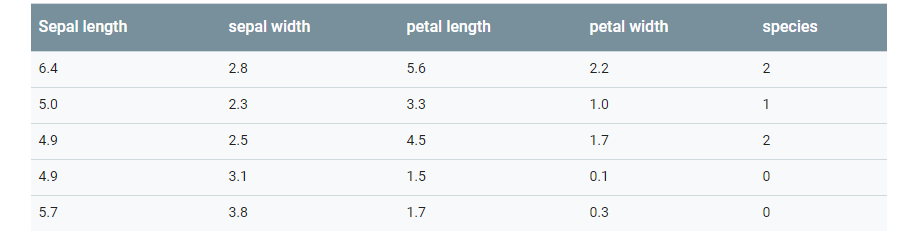
\includegraphics[scale=0.6]{img/iris}

De laatste kolom (species) noemt men een label, de eerste 4 kolommen noemen we features. Features zijn karakteristieken van een voorbeeld, terwijl een label hetgeen is wat we proberen te voorspellen. Een voorbeeld bestaat uit een set van features en een label voor één enkele bloem. De tabel hiervoor laat 5 voorbeelden zien uit de set van 120 voorbeelden.
Elke label is natuurlijk een string (“setosa”). Maar Machine Learning werkt op numerieke waarden. Dit is dus een probleem, daarom mappen we deze strings naar nummers.\newline
- 0 = setosa\newline
- 1 = versicolor\newline
- 2 = virginica\newline

\section{Models en training}
Een model is de relatie tussen functies en het label. Voor het Iris probleem definieert het model de relatie tussen de kelk- en bloembladmetingen en de voorspelde Iris-soort. Sommige eenvoudige modellen kunnen worden beschreven met een paar regels algebra, maar complexe modellen voor Machine Learning hebben een groot aantal parameters die moeilijk samen te vatten zijn. 

Zou je de relatie tussen de vier kenmerken en de Iris-soort kunnen bepalen zonder machine-learning te gebruiken? Dat wil zeggen, kunt u traditionele programmeertechnieken gebruiken om een model te maken? Kan zijn. Je zou lang genoeg met de dataset kunnen spelen om de juiste relaties van bloemblad- en kelkmetingen met bepaalde soorten te bepalen. Een goede benadering van Machine Learning bepaalt echter het model voor u. Dat wil zeggen, als u voldoende representatieve voorbeelden invoert in het juiste model voor het leren van een machine, bepaalt het programma de relatie tussen kelkbladen, bloembladen en soorten.

Training is het stadium van machine learning waarin het model geleidelijk wordt geoptimaliseerd (geleerd). Het Iris-probleem is een voorbeeld van machinaal onderwezen leren waarbij een model wordt getraind uit voorbeelden die labels bevatten. (In de non supervised machine-learning bevatten de voorbeelden geen labels, maar in plaats daarvan vindt het model meestal patronen tussen de functies.)

\section{Supervised Learning}

\section{Unsupervised Learning}







%%=============================================================================
%% Methodologie
%%=============================================================================

\chapter{Onderzoeksvragen}
\label{ch:Onderzoeksvragen}
In het volgende stuk van de bachelorproef volgt het beantwoorden van de onderzoeksvragen. Ik begin met de onderzoeksvraag te geven als titel en vervolgens ga ik aan de hand van de gegeven info op sites deze beantwoorden. 

\section{Zijn er andere technologieën die Machine Learning reeds toepassen voor churn of klantenbinding ?}
\label{ch:Onderzoeksvraag1}
Na wat zoeken op het web, ben ik tot de conclusie gekomen dat er toch al een aantal tools zijn die hiervoor gebruikt worden. Ik som ze hier even op met wat uitleg over de tools alsook de voor en nadelen hiervan. 

\subsubsection{Dataiku}
Op de Dataiku-website staat dat  de Data Science Studio is ontworpen als een hulpmiddel dat door iedereen gebruikt kan worden vanwege de open en transparante user-interface. Een van de grootste voordelen van de tool is dat iemand met helemaal geen programmeer ervaring hierin kan werken samen met iemand die een wat meer flexibel gebruik van de tool wil en zijn eigen code wil integreren. Hierdoor hebben mensen met verschillende vaardigheidsniveaus de mogelijkheid om een bijdrage te hebben aan het eindresultaat. Wat dus hoogst waarschijnlijk ook een beter eindresultaat zal zijn.[Dataiku review]

De tool probeert eenvoudige geïntegreerde toolboxes van populaire datamining-algoritmen op te nemen om veelvoorkomende problemen op te lossen, zoals linear regression voor wat meer eenvoudige voorspellingen. Omdat ze echter nogal simplistisch zijn kunnen ze niet worden afgestemd op specifieke behoeften. Hierdoor is het eigenlijk een voordeel dat het ook flexibiliteit biedt om de  gebruiker de mogelijkheid te geven om te coderen en dus een meer specifieke analyse te implementeren. Hoewel de tool geen vervanging is van de meer statistische technieken of menselijke vindingrijkheid, biedt het toch een degelijke basis van wat Data Science omvat, inclusief het gebruik van verschillende opties voor data-opruiming en gemeenschappelijke modelleringstechnieken.[Dataiku review]

Software Requirements

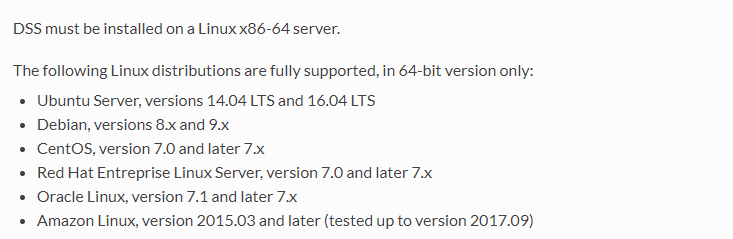
\includegraphics[scale=0.8]{img/software1}
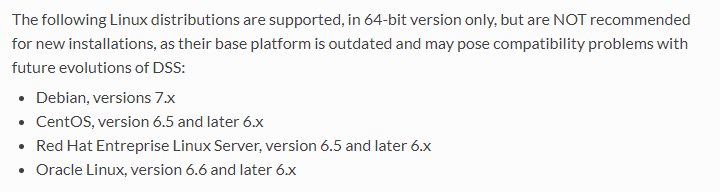
\includegraphics[scale=0.8]{img/software2}

Conclusie

Om Dataiku uit te proberen kan je op de site makkelijk videos en guides vinden die je snel opweg brengen met de tool. Om de tool te gebruiken heb je wel een Linux of Mac OS nodig. Aangezien ik Windows heb moet ik dus voor een review te maken eerst een virtual machine hebben. Als ik uiteindelijk deze tool ga gebruiken voor mijn eigen proof of concept. Dit heeft gelukkig een gratis versie die je altijd kan gebruiken maar deze heeft niet zo veel mogelijkheden als de betalende versie.

\subsection{IBM Watson Analytics}
Je hebt vragen, en je weet zeker dat de antwoorden te vinden zijn in jouw data. Dus wil je een eigen analyse doen. Maar je weet niet zo goed hoe je er aan moet beginnen. Je bent geen Data scientist. Maar je bent wel nieuwsgierig. Omdat je de middelen niet hebt, wacht je meestal op de analyses die je noèdig hebt van IT en dat kan weken duren. Stel je nu eens voor dat jij zelf analyses kan toepassen op jouw data. Hierin komt IBM Watson Analytics tot de redding. Dit is een smart data discovery solution in de cloud. Dat u begeleidt door het maken van analyses. Het automatiseert Data preparation, predictive modeling, en data visualization zodat je jouw nodige data snel hebt. Wachten op IT is dus niet meer nodig. Je moet geen Data Scientist zijn of een training volgen om met deze tool te werken.  

Op de IBM Watson Analytics site staat dat Watson Analytics een data-analyse en visualisatieservice is die je kan gebruiken om snel patronen en betekenis in uw gegevens te ontdekken, helemaal alleen. Met guided data discovery, automated predictive analytics en cognitive capabilities, kunt u bij manier van spreken een gesprek hebben met uw gegevens, en krijg je antwoorden die je makkelijk kan verstaan. Of je nu snel een trend moet zoeken, of een team hebt dat gevisualiseerde data moet krijgen in een dashboard. Het is allemaal mogelijk met Watson Analytics.  [Watson]

Software requirements\newline
Het enigste wat je hiervoor nodig hebt is een browser, de volgende browsers worden gesupport.\newline
-Apple Safari 9+
-Google Chrome 51+
-Microsoft Internet Explorer 11
- Mozilla Firefox 47+ and ESR 45+

Conclusie
Watson Analytics maakt gebruik van hun eigen REST API zodat je jouw eigen applicatie makkelijk kan integreren. Ook hier hebben ze op hun site een heleboel videos en guides die je kan terugvinden om snel op weg te geraken met deze tool. Voor dit te gebruiken moet je wel een \$30 betalen. Er is ook een gratis versie maar deze is maar een 14 dagen geldig. 

\subsection{Databricks}
Op hun site laten ze duidelijk zien welke problemen hun product kan oplossen. Ze laten in een video zien hoe A.I. en Big Data steeds meer en meer gebruikt wordt in bedrijven voor hun meer tijd te geven aan hun eigen inovatieve ideeën. Zoals het gebruik van geautomatiseerde image recognition, real time fraud detection of zelfs genome sequencing. Dit zorgt ervoor dat bedrijven anders gaan werken. Vervolgens laten ze een data engineer aan het woord. Data engineers transformeren en kuisen data op, Data scientists maken en testen machine learning models. Maar het is niet makkelijk om de Data engineers en scientists hun werk te vertalen naar business uitkomsten. Iedereen heeft verschillende vaardigheden. De een gebruikt Python, de ander Scala. Dit maakt het samenwerken moeilijker. Ze spenderen 90\% van hun tijd aan het maken van complexe data pipelines en dergelijke voor nog enkel maar de data klaar te stomen voor dit dan te analyseren. Hierdoor wordt beveiliging maar een na gedachte en innovatie een verre droom. Hiervoor is Databricks dan de ideale oplossing. Met hun unified data management zijn er dan geen problemen meer met data scientists en engineers hun verschillende vaardigheden. Ze maken gebruik van frameworks zoals TenserFlow. Hun clusters zitten in een cloud. Het is van de makers van Apache spark en is zo een 100 keer sneller dan hun open source stuk. Waardoor het team bijna direct data kan beschikbaar maken voor hun analisten. 

De software requirements kon ik niet vinden voor Databricks.

\section{Welke frameworks, visuele tools en scripting tools heb ik nodig om zelf zo een oplossing te bouwen?}
\label{ch:Onderzoeksvraag2}
Hoe maakt men nu zelf zo een oplossing? Dat is hier een van de vragen. Hoe begint men hieraan? We kunnen niet zomaar even op het web googelen, “How to make your own big data analyzer” of iets in die zin. Uiteindelijk bestaan er al een tal van frameworks en tools die hiervoor gebruikt kunnen worden. Zelfs tools die je misschien al kent maar waar je niet direct aan dacht. Zoals Excel. Maar waarom zouden we zelf tools nodig hebben ?

\subsubsection{Waarom tools gebruiken?}
Door het gebruik van tools kan men sneller en makkelijker werken.
Men kan sneller werken vanwege reeds geautomatiseerde stappen in het machine learning proces. Het alternatief is dat men alles van bij het begin moet maken .Wat veel langer kan duren dan gewoon een tool te gebruiken die men vindt op het web.
Het is makkelijker omdat er geen tijd nodig is voor zelf aan research te doen over hoe men bepaalde technieken moet gaan implementeren. Men kan in plaats van hieraan kostbare tijd te spenderen zoeken naar de juiste tool die jij nodig acht. Het alternatief is dat men een expert moet zijn in elke stap van het proces om het te kunnen implementeren. Wat veel onderzoek, oefenen vergt om de technieken te begrijpen.

\subsubsection{Platforms versus Libraries}
Er zijn veel Machine Learning tools, meer als genoeg waardoor je je al snel overwelmt voelt. Daarom is het nog geen slecht idee om Machine Learning tools te gaan onderverdelen in “Platforms” en “Libraries”. Een platform biedt alles wat je nodig hebt om een project te laten draaien. Terwijl een library enkele delen van wat je nodig hebt voor een project te starten aanbiedt. Dit is geen perfecte onderscheiding, aangezien sommige platforms soms libraries zijn en sommige libraries een grafische user interface geven. Voor ons kan dit toch wel een goede scheidingslijn vormen.

\textbf{1. Machine Learning Platform} \newline
Een Machine Learning platform biedt mogelijkheden om een ML project van begin tot eind te voltooien. Namelijk, sommige data-analyse, data-voorbereiding,modellering en algoritme evaluatie en selectie
Kenmerken van machine learning platforms zijn:\newline
-Ze bieden mogelijkheden die in elke stap nodig zijn in een machine learning project.\newline
-De interface mag grafisch zijn, command line of een combinatie van beiden.\newline
-Ze bieden een losse koppeling van functies waardoor u de stukken aan elkaar moet knopen voor uw specifiek project \newline
-Ze zijn op maat gemaakt voor algemeen gebruik in plaats van snelheid, schaalbaarheid of nauwkeurigheid.\newline

Voorbeelden van Machine Learning platforms\newline
-WEKA Machine learning workbench\newline
-R Platform\newline
-Pandas \newline

\textbf{2. Machine Learning Library} \newline
Een machine learning library biedt mogelijkheden voor het voltooien van een deel van een Machine Learning project. Een library kan bijvoorbeeld een verzameling modelleringsalgoritmen bieden
Kenmerken van machine learning libraries zijn:\newline
-Ze bieden een specifieke mogelijkheid voor een of meer stappen in een Machine Learning project.\newline
-De Interface is meestal een API(Een verzameling definities op basis waarvan een computerprogramma kan communiceren met een ander programma of onderdeel)\newline
-Ze zijn afgestemd op een specifiek gebruik, probleemtype of omgeving.\newline
Voorbeelden van machine learning libraries zijn:\newline
-Scikit-learn (Python)\newline
-JSAT (Java)\newline
-Accord Framework (.NET)

\subsection{Machine Learning Tool interfaces}
Een andere handige manier om na te denken over machine learning tools is door de interface die ze bieden. Dit kan verwarrend zijn, omdat sommige tools meerdere interfaces bieden. Niettemin biedt het een startpunt en misschien een punt van differentiatie om u te helpen bij het kiezen van een machine learning tool.
Hieronder zijn enkele voorbeelden van veelgebruikte interfaces.\newline
\textbf{1.Graphical User Interface (GUI)}\newline
Machine learning tools bieden een Graphical User Interface , ”point and click” en een focus op visualisatie. 
De voordelen van een grafische gebruikersinterface zijn:\newline
- Stelt minder technische gebruikers in staat om aan ML te doen.\newline
- Focus op het proces en hoe je het meeste uit ML technieken kan halen.\newline
- De gebruiker krijgt een meer gestructureerd beeld voor zich.

Enkele voorbeelden van ML tools met een grafische interface zijn:\newline
-KNIME \newline
-RapidMiner \newline
-Orange \newline

\textbf{2. Command Line Interface} \newline
ML tools bieden een command line interface met command line programma’s, command line parameterisatie met een focus op input en output. De voordelen van command line user interface zijn: \newline
-Hiermee kunnen mensen die goed overweg kunnen met de command line ook makkelijk door hun ML projecten. \newline
-Biedt veel kleine gerichte programma’s of programma modes voor specifieke subtaken van een ML project. \newline
-Stelt machine learning taken af op basis van de vereiste input en output die moet worden gegenereerd.\newline
Een paar voorbeelden van ML tools voor een command line interface zijn:\newline
-Waffles\newline
-Weka Machine Learning Workbench

\textbf{3. Application Programming Interface(API})\newline
Machine learning tools kunnen u ook een API aanbieden waarmee u zelf kunt bepalen welke elementen u moet gebruiken en hoe u ze precies kunt gebruiken binnen uw eigen programma’s. De voordelen voor API zijn:\newline
-Je kan machine learning integreren in eigen software projecten.\newline
-Hiermee kan je jouw eigen machine learning tools maken.\newline
-Biedt flexibiliteit om eigen processen en automatiseringen te gebruiken voor machine learning projecten.\newline
-Laat toe om uw eigen methoden te combineren met die van de libraries.\newline
Voorbeelden van machine learning tools met API\newline
-Pylearn2 (python)\newline
-Deeplearing4j (java)\newline
-LIBSVM (C)\newline
-TenserFlow(Java, Go, C)\newline

\subsection{Local versus Remote Machine Learning Tools}
Een laatste manier om machine learning tools te vergelijken is door na te gaan of de tool local of remote is
Een local tool is een tool die u lokaal kunt downloaden, installeren en gebruiken, waarbij als externe tool op een externe server wordt uitgevoerd. Dit onderscheid kan ook een beetje troebel zijn omdat sommige tools op een lokale of externe manier kunnen worden uitgevoerd. En uiteindelijk kunt u bijna elk tool als een gehoste oplossing op uw eigen servers configureren. Toch kan dit nog een nuttig onderscheid zijn.

\textbf{1. Local Tools} \newline
Een lokale tool wordt dus zoals de naam zegt, lokaal gedraaid. \newline
- Het wordt op maat gemaakt voor gegevens en algoritmen in het geheugen. \newline
- Je hebt controle over runconfiguratie parameterization. \newline
- U kan het integreren in uw eigen systeem om aan uw behoeften te voldoen. \newline

Voorbeelden van lokale tools zijn:  \newline
Shogun Library (C++) \newline
GoLearn (Go) \newline

\textbf{2. Remote Tools} \newline
Een remote tool wordt gehost op een server en wordt opgeroepen vanuit een lokale omgeving. Deze tools worden vaak Machine Learning as a Service (MLaaS) genoemd. \newline
- Speciaal gemaakt voor uitbereiding, kan worden uitgevoerd op grotere datasets. \newline
- Werkt op meerdere systemen, meerdere kernen en shared memory. \newline
- Minder algoritmen vanwege de aanpassingen die nodig zijn om op schaal te werken. \newline
- Eenvoudigere interfaces , waardoor er minder controle is over run configuratie en parameter aanpassingen van algoritmen. \newline
- Geïntegreerd in uw lokale omgeving via remote procedure calls. \newline
Voorbeelden van remote tools: \newline
- Google Prediction API \newline
- AWS Machine Learning \newline
- Microsoft Azure Machine Learning.


\subsection{Samenvatting}
In dit deel hebben we ontdekt waarom tools dus zo belangrijk zijn als men aan machine learning wil doen. Zonder al deze handige ML tools zouden we al deze technieken zelf moeten maken en implementeren, wat een zeer goede expertise vereist. In dit stuk heeft men ook aangetoond dat er verschillende soorten ML tools zijn die men kan onderscheiden.\newline
-Platforms versus Libraries \newline
- Graphical User Interfaces versus Command-Line Interface Versus Application Programming Interfaces \newline
- Local versus Remote 

\subsection{Conclusie}
Zoals men kan zien zijn er zeer veel tools waaruit men kan kiezen. Met elk hun sterktes en zwaktes, elke tool dat werd opgenoemd heeft men niet apart uitgelegd vanwege het aantal. Hieruit kunnen we dus goed beslissen welke soort tool we nodig zullen hebben. En vervolgens daaruit dan selecteren welke tool we uiteindelijk gaan gebruiken.\newline\newline
\textbf{Platform of libraries?}\newline
een platform is een kant en klare tool eigenlijk wat niet veel ruimte laat voor eigen modificaties. Wat ons kan belemmeren. Bij deze kiest men voor  libraries\newline
\textbf{GUI, Command Line of API?}\newline
Alhoewel het gebruik van GUI tools makkelijker is voor beginners, gaat men toch kiezen voor API. Kiest men toch voor API. De API laat toe om zelf een machine learning tool te maken. En dat is uiteindelijk wat men wou bereiken in deze bachelorproef.
\textbf{Local of remote ?} \newline
Dit maakt niet veel uit voor deze bachelorproef. Men gaat hier gaan voor hetgeen wat men het eenvoudigste vindt. Local.

De tool definitie die we hebben gekozen is : Library , API, Local
Na wat zoeken op het web heeft men al snel een paar tools gevonden die aan onze definitie voldoet.

\subsection{Tenserflow}
Algemene informatie over tenserflow

\subsection{Deeplearning4j} 
Algemene informatie over Deeplearning4j

\subsection{Conclusie}
vergelijken

\section{Welke Dataset gaan we gebruiken en hoe verkrijg ik deze data?}
De manier waarop men deze vraag moet interpreteren is eigenlijk welke parameters/variabelen hebben we zeker nodig in een data set om churn te kunnen voorspellen? Eerst en vooral moet men besluiten of er gaat gewerkt worden met supervised of unsupervised learning. In de literatuur studie heeft men hierover reeds het verschil uitgelegd. \newline
Supervised Machine Learning is wanneer we input variabelen en output variabelen hebben. Het doel is dat men de functie zo willen uitvoeren dat we met een nieuwe input waarde de output waarde kunnen voorspellen\newline
Unsupervised Machine Learning is wanneer men enkel input waarden heeft zonder de output waarden. Het doel hiervan is dat men meer over de input data te weten komt.\newline
Aangezien we niet onmiddellijk meer informatie willen over de input waarden maar wel willen voorspellen welke de output zal zijn, namelijk of een klant gaat churnen ,ja of neen ,1 of 0. Zou men graag een data set willen waar het resultaat ook aanwezig is in de data set.\newline
Dus men kan al één conclusie trekken. De dataset moet een label hebben. In de vorm van Churn ja of neen.\newline
Voor aan gesuperviseerd leren te doen moet men niet enkel output hebben. Daarmee zijn we niet veel. Er moet ook nog input aanwezig zijn. Deze input is eigenlijk alle data wat we weten over deze ene klant. Elke bedrijf segmenteert zijn klanten. In de literatuur studie ziet men hoe men klanten moet gaan onderverdelen. Dankzij model gebaseerde segmentatie kan men makkelijk heel veel variabelen als input meegeven. Betalingsmethoden, tijd, locatie, prijs, hoeveelheid gekocht, korting, het weer, enz…

\subsection{Telco-Customer-data set}
Deze dataset bevat info die ons kan helpen om het gedrag van klanten te gaan voorspellen. Deze data set heeft men gevonden op de IBM Watson Analytics site in een tutorial. In de tutorial gaat het als volgt. Een telecom bedrijf is bezorgd over het aantal klanten dat ze verliezen aan hun concurrentie. Ze willen te weten komen wie er gaat vertrekken. In het voorbeeld op de site moet je u inbeelden dat jij de analist bent in hun bedrijf en dat jij dit moet uitzoeken.

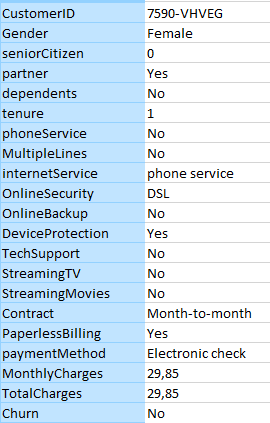
\includegraphics[scale=0.8]{img/dataset}

De data set heeft informatie over

•	De klanten die het bedrijf zijn verlaten. De laatste kolom Churn. \newline
•	Services waar elke klant voor geabonneerd is, phones,multiple lines, internet,online security,online backup,device,protection,tech support, 		 streaming TV en movies. \newline
•	-Profiel informatie van de klant, hoelang ze al klant zijn,contract,payment method,paperless billing, monthly charges, en total charges\newline
•	-Demographic info over de klanten gender, age, range en of ze partners en dependents hebben.

Hier ziet men eigenlijk al goed dat deze data set een tal van onze gewenste variabelen bevat.
Maar we moeten onze dataset nog opschonen. Dit komt voor in de proof of concept.

\section{Welk Model dien ik hiervoor op te zetten?}

\section{Kies ik beter scripting tools zoals python?}












%%=============================================================================
%% Proof of Concept
%%=============================================================================

\chapter{Proof of Concept}
\label{ch:Proof of concept}


\section{specificaties van mijn systeem}

\section{installatie van TenserFlow}
Voor men begon met de proof of concept moet men eerst TenserFlow installeren. Op de site van TenserFlow staat er een handleiding hoe men TenserFlow moet installeren, en wat voor versie van TenserFlow men wilt installeren. Men kan kiezen tussen 2 versies:
TenserFlow met enkel CPU support Dit is voor de systemen die geen NVIDIA GPU hebben. Dit is een versie die makkelijker is om te installeren en men raadt ons aan om toch deze versie te installeren ook al hebben we een NVIDIA GPU
TenserFlow met GPU support. De TenserFlow programma’s werken sneller op hun GPU dan op een CPU, daarvoor als het systeem een NVIDIA GPU heeft met de nodige voorwaarden die onderaan ook vermeld staan en als men performance-critical applications moeten draaien, dan moeten we deze versie toch installeren.

•	CUDA Toolkit 9.0, je moet ook de nodige Cuba pathnames in de environment variabele toevoegen\newline
•	NVIDIA drivers die gelinkt zijn aan de CUDE Toolkit 9.0\newline
•	cuDNN v7.0 


%%=============================================================================
%% Proof of Concept
%%=============================================================================

\chapter{Bronnen}
\label{ch:Bronnen}


\section{bronnen}

\begin{verbatim}
https://teamloyalty.nl/kennis/wat-is-klantenbinding/ 
https://hbr.org/2010/07/stop-trying-to-delight-your-customers 
https://www.superoffice.com/blog/reduce-customer-churn/ 
https://medium.com/machine-learning-for-humans/why-machine-learning-matters-6164faf1df12 
https://www.tensorflow.org/get_started/get_started_for_beginners https://en.wikipedia.org/wiki/Iris_flower_data_set 
https://medium.com/big-data-driving-innovation/reviewing-data-science-tool-dataiku-f571a250ffb9 https://amplitude.com/blog/2016/04/21/thinking-building-analytics-dont https://machinelearningmastery.com/machine-learning-tools/
https://cdn2.hubspot.net/hubfs/2123903/PDF/Whitepaper/guidebook-churn-prediction.pdf 
https://www.ibm.com/communities/analytics/watson-analytics-blog/predictive-insights-in-the-telco-customer-churn-data-set/ 
http://www.ronaldvanloon.com/machine-learning-explained-understanding-supervised-unsupervised-and-reinforcement-learning/ 
https://www.dataiku.com/dss/features/machine-learning/ 

\end{verbatim}





% Voeg hier je eigen hoofdstukken toe die de ``corpus'' van je bachelorproef
% vormen. De structuur en titels hangen af van je eigen onderzoek. Je kan bv.
% elke fase in je onderzoek in een apart hoofdstuk bespreken.

%\input{...}
%\input{...}
%...

%%=============================================================================
%% Conclusie
%%=============================================================================

\chapter{Conclusie}
\label{ch:conclusie}

%% TODO: Trek een duidelijke conclusie, in de vorm van een antwoord op de
%% onderzoeksvra(a)g(en). Wat was jouw bijdrage aan het onderzoeksdomein en
%% hoe biedt dit meerwaarde aan het vakgebied/doelgroep? Reflecteer kritisch
%% over het resultaat. Had je deze uitkomst verwacht? Zijn er zaken die nog
%% niet duidelijk zijn? Heeft het onderzoek geleid tot nieuwe vragen die
%% uitnodigen tot verder onderzoek?

\lipsum[76-80]



%%=============================================================================
%% Bijlagen
%%=============================================================================

\appendix

%%---------- Onderzoeksvoorstel -----------------------------------------------

\chapter{Onderzoeksvoorstel}

Het onderwerp van deze bachelorproef is gebaseerd op een onderzoeksvoorstel dat vooraf werd beoordeeld door de promotor. Dat voorstel is opgenomen in deze bijlage.

% Verwijzing naar het bestand met de inhoud van het onderzoeksvoorstel
%---------- Inleiding ---------------------------------------------------------

\section{Introductie} % The \section*{} command stops section numbering
\label{sec:introductie}

Hier introduceer je werk. Je hoeft hier nog niet te technisch te gaan.

Je beschrijft zeker:

\begin{itemize}
  \item de probleemstelling en context
  \item de motivatie en relevantie voor het onderzoek
  \item de doelstelling en onderzoeksvraag/-vragen
\end{itemize}

%---------- Stand van zaken ---------------------------------------------------

\section{State-of-the-art}
\label{sec:state-of-the-art}

Hier beschrijf je de \emph{state-of-the-art} rondom je gekozen onderzoeksdomein. Dit kan bijvoorbeeld een literatuurstudie zijn. Je mag de titel van deze sectie ook aanpassen (literatuurstudie, stand van zaken, enz.). Zijn er al gelijkaardige onderzoeken gevoerd? Wat concluderen ze? Wat is het verschil met jouw onderzoek? Wat is de relevantie met jouw onderzoek?

Verwijs bij elke introductie van een term of bewering over het domein naar de vakliteratuur, bijvoorbeeld~\autocite{Doll1954}! Denk zeker goed na welke werken je refereert en waarom.

% Voor literatuurverwijzingen zijn er twee belangrijke commando's:
% \autocite{KEY} => (Auteur, jaartal) Gebruik dit als de naam van de auteur
%   geen onderdeel is van de zin.
% \textcite{KEY} => Auteur (jaartal)  Gebruik dit als de auteursnaam wel een
%   functie heeft in de zin (bv. ``Uit onderzoek door Doll & Hill (1954) bleek
%   ...'')

Je mag gerust gebruik maken van subsecties in dit onderdeel.

%---------- Methodologie ------------------------------------------------------
\section{Methodologie}
\label{sec:methodologie}

Hier beschrijf je hoe je van plan bent het onderzoek te voeren. Welke onderzoekstechniek ga je toepassen om elk van je onderzoeksvragen te beantwoorden? Gebruik je hiervoor experimenten, vragenlijsten, simulaties? Je beschrijft ook al welke tools je denkt hiervoor te gebruiken of te ontwikkelen.

%---------- Verwachte resultaten ----------------------------------------------
\section{Verwachte resultaten}
\label{sec:verwachte_resultaten}

Hier beschrijf je welke resultaten je verwacht. Als je metingen en simulaties uitvoert, kan je hier al mock-ups maken van de grafieken samen met de verwachte conclusies. Benoem zeker al je assen en de stukken van de grafiek die je gaat gebruiken. Dit zorgt ervoor dat je concreet weet hoe je je data gaat moeten structureren.

%---------- Verwachte conclusies ----------------------------------------------
\section{Verwachte conclusies}
\label{sec:verwachte_conclusies}

Hier beschrijf je wat je verwacht uit je onderzoek, met de motivatie waarom. Het is \textbf{niet} erg indien uit je onderzoek andere resultaten en conclusies vloeien dan dat je hier beschrijft: het is dan juist interessant om te onderzoeken waarom jouw hypothesen niet overeenkomen met de resultaten.



%%---------- Andere bijlagen --------------------------------------------------
% TODO: Voeg hier eventuele andere bijlagen toe
%\input{...}

%%---------- Referentielijst --------------------------------------------------

\printbibliography[heading=bibintoc]
%\addcontentsline{toc}{chapter}{\textcolor{maincolor}{\IfLanguageName{dutch}{Bibliografie}{Bibliography}}}

\end{document}
